% Options for packages loaded elsewhere
\PassOptionsToPackage{unicode}{hyperref}
\PassOptionsToPackage{hyphens}{url}
\PassOptionsToPackage{dvipsnames,svgnames,x11names}{xcolor}
%
\documentclass[
  11pt,
]{article}
\usepackage{amsmath,amssymb}
\usepackage{setspace}
\usepackage{iftex}
\ifPDFTeX
  \usepackage[T1]{fontenc}
  \usepackage[utf8]{inputenc}
  \usepackage{textcomp} % provide euro and other symbols
\else % if luatex or xetex
  \usepackage{unicode-math} % this also loads fontspec
  \defaultfontfeatures{Scale=MatchLowercase}
  \defaultfontfeatures[\rmfamily]{Ligatures=TeX,Scale=1}
\fi
\usepackage{lmodern}
\ifPDFTeX\else
  % xetex/luatex font selection
    \setmainfont[]{Times New Roman}
\fi
% Use upquote if available, for straight quotes in verbatim environments
\IfFileExists{upquote.sty}{\usepackage{upquote}}{}
\IfFileExists{microtype.sty}{% use microtype if available
  \usepackage[]{microtype}
  \UseMicrotypeSet[protrusion]{basicmath} % disable protrusion for tt fonts
}{}
\makeatletter
\@ifundefined{KOMAClassName}{% if non-KOMA class
  \IfFileExists{parskip.sty}{%
    \usepackage{parskip}
  }{% else
    \setlength{\parindent}{0pt}
    \setlength{\parskip}{6pt plus 2pt minus 1pt}}
}{% if KOMA class
  \KOMAoptions{parskip=half}}
\makeatother
\usepackage{xcolor}
\usepackage[margin=2cm]{geometry}
\usepackage{longtable,booktabs,array}
\usepackage{calc} % for calculating minipage widths
% Correct order of tables after \paragraph or \subparagraph
\usepackage{etoolbox}
\makeatletter
\patchcmd\longtable{\par}{\if@noskipsec\mbox{}\fi\par}{}{}
\makeatother
% Allow footnotes in longtable head/foot
\IfFileExists{footnotehyper.sty}{\usepackage{footnotehyper}}{\usepackage{footnote}}
\makesavenoteenv{longtable}
\usepackage{graphicx}
\makeatletter
\newsavebox\pandoc@box
\newcommand*\pandocbounded[1]{% scales image to fit in text height/width
  \sbox\pandoc@box{#1}%
  \Gscale@div\@tempa{\textheight}{\dimexpr\ht\pandoc@box+\dp\pandoc@box\relax}%
  \Gscale@div\@tempb{\linewidth}{\wd\pandoc@box}%
  \ifdim\@tempb\p@<\@tempa\p@\let\@tempa\@tempb\fi% select the smaller of both
  \ifdim\@tempa\p@<\p@\scalebox{\@tempa}{\usebox\pandoc@box}%
  \else\usebox{\pandoc@box}%
  \fi%
}
% Set default figure placement to htbp
\def\fps@figure{htbp}
\makeatother
\setlength{\emergencystretch}{3em} % prevent overfull lines
\providecommand{\tightlist}{%
  \setlength{\itemsep}{0pt}\setlength{\parskip}{0pt}}
\setcounter{secnumdepth}{5}
% definitions for citeproc citations
\NewDocumentCommand\citeproctext{}{}
\NewDocumentCommand\citeproc{mm}{%
  \begingroup\def\citeproctext{#2}\cite{#1}\endgroup}
\makeatletter
 % allow citations to break across lines
 \let\@cite@ofmt\@firstofone
 % avoid brackets around text for \cite:
 \def\@biblabel#1{}
 \def\@cite#1#2{{#1\if@tempswa , #2\fi}}
\makeatother
\newlength{\cslhangindent}
\setlength{\cslhangindent}{1.5em}
\newlength{\csllabelwidth}
\setlength{\csllabelwidth}{3em}
\newenvironment{CSLReferences}[2] % #1 hanging-indent, #2 entry-spacing
 {\begin{list}{}{%
  \setlength{\itemindent}{0pt}
  \setlength{\leftmargin}{0pt}
  \setlength{\parsep}{0pt}
  % turn on hanging indent if param 1 is 1
  \ifodd #1
   \setlength{\leftmargin}{\cslhangindent}
   \setlength{\itemindent}{-1\cslhangindent}
  \fi
  % set entry spacing
  \setlength{\itemsep}{#2\baselineskip}}}
 {\end{list}}
\usepackage{calc}
\newcommand{\CSLBlock}[1]{\hfill\break\parbox[t]{\linewidth}{\strut\ignorespaces#1\strut}}
\newcommand{\CSLLeftMargin}[1]{\parbox[t]{\csllabelwidth}{\strut#1\strut}}
\newcommand{\CSLRightInline}[1]{\parbox[t]{\linewidth - \csllabelwidth}{\strut#1\strut}}
\newcommand{\CSLIndent}[1]{\hspace{\cslhangindent}#1}
% Break sections into new page
\usepackage{titlesec}
\newcommand{\sectionbreak}{\clearpage}

% Table caption 
\usepackage{caption} 
\captionsetup[table]{skip=8pt}

% Table packages
\usepackage{longtable}
\usepackage{array}
\usepackage{multirow}
\usepackage{wrapfig}
\usepackage{float}
\usepackage{colortbl}
\usepackage{pdflscape}
\usepackage{tabu}
\usepackage{threeparttable}
\usepackage{threeparttablex}
\usepackage[normalem]{ulem}
\usepackage{makecell}
\usepackage{xcolor}

% Move all figures at the end
\usepackage[nolists, nomarkers]{endfloat}
\DeclareDelayedFloatFlavour*{longtable}{table}

%\graphicspath{}

\usepackage{booktabs}
\usepackage{longtable}
\usepackage{array}
\usepackage{multirow}
\usepackage{wrapfig}
\usepackage{float}
\usepackage{colortbl}
\usepackage{pdflscape}
\usepackage{tabu}
\usepackage{threeparttable}
\usepackage{threeparttablex}
\usepackage[normalem]{ulem}
\usepackage{makecell}
\usepackage{xcolor}
\usepackage{bookmark}
\IfFileExists{xurl.sty}{\usepackage{xurl}}{} % add URL line breaks if available
\urlstyle{same}
\hypersetup{
  pdftitle={Exploring the Role of AI Chatbots in K-12 Education: A Comparative Study of Socratic and Non-Socratic Approaches},
  pdfauthor={Andrea Blasco1,; Vicky Charisi1,2,},
  colorlinks=true,
  linkcolor={Maroon},
  filecolor={Maroon},
  citecolor={Blue},
  urlcolor={Blue},
  pdfcreator={LaTeX via pandoc}}

\title{Exploring the Role of AI Chatbots in K-12 Education: A Comparative Study of Socratic and Non-Socratic Approaches}
\author{Andrea Blasco\textsuperscript{1,*} \and Vicky Charisi\textsuperscript{1,2,*}}
\date{This version: June 03, 2025}

\begin{document}
\maketitle

\setstretch{2}
\textsuperscript{1} European Commission, Joint Research Centre, Brussels, Belgium\\
\textsuperscript{2} Harvard University, Berkman Klein Center, Cambridge, MA, USA

\textsuperscript{*} Correspondence: \href{mailto:andrea.blasco@ec.europa.eu}{Andrea Blasco \textless{}\href{mailto:andrea.blasco@ec.europa.eu}{\nolinkurl{andrea.blasco@ec.europa.eu}}\textgreater{}}, \href{mailto:vcharisi@law.harvard.edu}{Vicky Charisi \textless{}\href{mailto:vcharisi@law.harvard.edu}{\nolinkurl{vcharisi@law.harvard.edu}}\textgreater{}}

\section*{Highlights}\label{highlights}
\addcontentsline{toc}{section}{Highlights}

\begin{itemize}
\item
  An experiment was conducted where K-12 students used AI chatbots to solve school-related problems.
\item
  Two AI chatbot approaches were tested: one provided incremental guidance to encourage critical thinking (``Socratic''), while the other offered immediate solutions (``non-Socratic'').
\item
  Results showed that AI-generated explanations improved students' performance over solutions without them, highlighting the value of AI-generated guidance.
\item
  Participants engaged more frequently with the Socratic AI, though this did not result in improved performance compared to the non-Socratic AI.
\item
  While students found interactions with the AI useful, they perceived the Socratic AI as less helpful overall.
\item
  The findings highlight challenges in designing AI tutors that effectively foster critical thinking while maintaining student satisfaction, raising concerns about their adoption in educational settings.
\end{itemize}

\section*{Abstract}\label{abstract}
\addcontentsline{toc}{section}{Abstract}

How does integrating large language models (LLMs) into classroom activities influence students' learning? To address this question, we conducted a randomized experiment comparing two distinct chatbot approaches: one designed to encourage critical thinking through incremental guidance (``Socratic AI'') and another providing immediate solutions (``non-Socratic AI''). The study involved students aged 14 to 16, who engaged in various school-related tasks under these experimental conditions. Students' attitudes were measured through self-reported surveys. Results indicated that AI-generated explanations significantly improved students' performance over solutions provided without such explanations, highlighting the benefits of step-by-step guidance. The Socratic AI approach fostered significantly greater engagement and interaction. However, it did not achieve significant improvements in learning, and a higher fraction of students perceived it as less helpful. Furthermore, despite students generally perceiving AI assistance as beneficial, they exhibited limited retention, failing to apply learned concepts to new situations when we removed AI assistance. These findings contribute to the ongoing debate on integrating LLM-powered chatbots in education, highlighting key challenges in designing AI tutors that effectively foster critical thinking while maintaining student satisfaction, raising concerns about their adoption in educational settings.

\textbf{Keywords}: artificial intelligence; large language models; learning; education policy; experiment, k-12

\section{Introduction}\label{introduction}

Integrating artificial intelligence (AI) into educational settings has been debated for over three decades (\citeproc{ref-roll2016evolution}{Roll and Wylie 2016}). Recent advances in generative AI and large language model (LLM) chatbots have opened even more possibilities for improvements in educational practices (\citeproc{ref-yan2024promises}{Yan, Greiff, et al. 2024}; \citeproc{ref-kasneci2023chatgpt}{Kasneci et al. 2023}; \citeproc{ref-tlili2023if}{Tlili et al. 2023}). Although LLMs mimic human intelligence, their applications extend beyond imitation and include a range of educational tasks: facilitating problem-solving (\citeproc{ref-urban2024chatgpt}{Urban et al. 2024}), language learning (\citeproc{ref-derakhshan2024chatgpt}{Derakhshan and Ghiasvand 2024}; \citeproc{ref-song2023enhancing}{Song and Song 2023}), or evaluation of students' work (\citeproc{ref-henkel2024can}{Henkel et al. 2024}). However, the impact of these applications on students' learning remains controversial, with proponents highlighting potential benefits and critics cautioning about risks and drawbacks. This study addresses two critical aspects of AI integration in education: the effectiveness of AI-generated explanations and the optimal modes of interaction between AI and students, specifically whether Socratic or alternative approaches yield better outcomes.

A key advancement over previous AI systems is that LLMs can generate step-by-step solutions to accompany their responses to students' queries. This study investigates how this ability influences students' interactions and helps them enhance their problem-solving skills. Specifically, we first examine the impact of AI explanations on students' performance in a numerical estimation task and their assessment of the accuracy of AI-generated predictions. Then, we test two approaches to access these explanations through AI chatbots: one approach that encourages critical thinking through incremental guidance (``Socratic AI'') and another providing immediate solutions (``non-Socratic AI'').

Previous research has shown that explanations can foster children's causal learning and contribute to the development of their scientific reasoning (\citeproc{ref-dejong1986explanation}{DeJong and Mooney 1986}; \citeproc{ref-legare2014contributions}{Legare 2014}; \citeproc{ref-danovitch2021mind}{Danovitch et al. 2021}). Similarly, explanations generated by LLMs may guide students in their problem-solving, for example, by decomposing a numerical estimation task into more manageable steps, such as considering heuristics or approximations. However, LLMs can also generate inaccuracies and flawed reasoning (\citeproc{ref-saxton2019analysing}{Saxton et al. 2019}; \citeproc{ref-kalyan2021how}{Kalyan et al. 2021}; \citeproc{ref-hendrycks2021measuring}{Hendrycks et al. 2021}), misleading students if followed without scrutiny. Understanding this dual role of AI explanations as a valuable educational tool and a potential source of misinformation leads to our first research question (RQ):

\textbf{RQ-1: Do AI-generated explanations enhance learning by providing insights, or do they risk impairing students' critical thinking by presenting inaccurate reasoning as authoritative?}

The study also aims to explore how different modes of student-AI interaction more broadly influence students' performance and perceptions, of which providing explanations is one key element. Specifically, we contrast two fundamental approaches: the ``Socratic'' and ``non-Socratic'' methods. The Socratic approach, inspired by the Socratic teaching method (\citeproc{ref-lam2011socratic}{Lam 2011}; \citeproc{ref-dalim2022promoting}{Dalim, Ishak, and Hamzah 2022}), engages students through an argumentative dialogue where the AI tutor asks thought-provoking questions to stimulate critical thinking and self-reflection (\citeproc{ref-wilberding2021socratic}{Wilberding 2021}). This method encourages students to think critically and arrive at their answers rather than relying on the AI-generated solution, thus helping students gain more confidence in their reasoning (\citeproc{ref-cleveland2015beyond}{Cleveland 2015}). In contrast, the non-Socratic approach directly answers students' queries without necessarily engaging them in a dialogue or exploration.

The Socratic approach has recently gained considerable attention in the context of AI tutoring in education. Notably, Khan Academy has developed its AI tutor, Khanmigo, based on these principles, aiming to foster critical thinking and engagement in learners.\footnote{\url{https://docsbot.ai/prompts/education/khanmigo-lite-socratic-tutor}}. Several commentators have argued that the Socratic method is particularly effective for designing AI tutors for children, as it enhances critical thinking and discourages students from copying AI-generated responses without scrutiny (\citeproc{ref-lara2020artificial}{Lara and Deckers 2020}).\footnote{See also \url{https://research.gatech.edu/ai-oral-assessment-tool-uses-socratic-method-test-students-knowledge}} This debate raises the following research question:

\textbf{RQ-2: Do student-AI interactions guided by the Socratic method promote deeper critical thinking and enhance students' confidence in their answers?}

Another objective of comparing Socratic and non-Socratic AI is to assess the extent of ``user satisfaction'' among students. Regardless of its academic benefits, Socratic AI could find limited application if students find interacting with Socratic AI chatbots unengaging or frustrating. Negative interactions or perceptions might drive students away in favour of more straightforward (non-Socratic) tools that provide direct answers, such as ChatGPT. Therefore, aligning educational benefits with user satisfaction is crucial for ensuring the long-term adoption of AI learning tools. This leads to our last research question:

\textbf{RQ-3: How do students perceive the helpfulness of Socratic AI compared to non-Socratic AI?}

By focusing on the impact of AI explanations and the Socratic AI approach on students' critical thinking, we aim to contribute to a growing literature about integrating AI into education. Recent research on AI chatbots and LLMs indicates significant potential for improving student learning outcomes. A meta-analysis of 24 randomised studies highlights the positive impact of chatbots, especially on student productivity and learning engagement (\citeproc{ref-wu2024ai}{Wu and Yu 2024}). However, several studies are more cautious about the benefits, partly due to concerns that AI might encourage cheating, over-reliance, or superficial understanding, which are challenging to measure in short-term studies (\citeproc{ref-lee2024cheating}{Lee et al. 2024}). Additional studies on LLMs' impact on academic integrity show that students and teachers struggle to differentiate between human and AI-generated text, raising risks of increased academic dishonesty and eroded trust (\citeproc{ref-yusuf2024generative}{Yusuf, Pervin, and Román-González 2024}; \citeproc{ref-eke2023chatgpt}{Eke 2023}). Furthermore, as LLMs continue to evolve, students and educators may lack the skills to leverage them effectively, which could result in missed educational opportunities (\citeproc{ref-kaplan2023generative}{Kaplan-Rakowski et al. 2023}).

The ethical and societal implications of LLMs in education are also complex. Issues such as bias, privacy, surveillance, and autonomy persist, especially in K-12 contexts, where the impact of algorithmic decisions on young learners' agency and privacy can be profound (\citeproc{ref-williams2024ethical}{Williams 2024}). LLMs introduce unique challenges, notably in alignment, where the system's goals may not align fully with educational objectives, despite companies' efforts to mitigate such risks through fine-tuning and reinforcement learning (\citeproc{ref-gabriel2020artificial}{Gabriel 2020}). Concerns also extend to students' digital well-being, as AI in education could inadvertently contribute to unhealthy digital habits and reliance on AI assistance over critical thinking (\citeproc{ref-weidinger2022taxonomy}{Weidinger et al. 2022}). Given these multidimensional impacts, further research is needed to optimise AI's role in education, balancing short-term learning gains with long-term skill development and ethical considerations.

Research in the field of human-AI combinations does not indicate consensus in terms of its effectiveness. For example, using a meta-analysis of studies published between 2020 and 2023, Vaccaro, Almaatouq, and Malone (\citeproc{ref-vaccaro2024combinations}{2024}) finds that, on average, human-AI combinations performed significantly worse than the best of humans or AI alone. On the other hand, Li et al. (\citeproc{ref-li2024explanatory}{2024}) uses a sample of 200 Chinese students to show significant correlations between human--computer interactions, perceived usefulness and students' skills. Understanding these associations can help institutions design better AI courses and more effective integration of AI in education.

This study advances this literature on human-AI collaboration in educational contexts by examining the role of step-by-step reasoning and the impact of different modes of AI interaction. Additionally, it contributes to ongoing research exploring the factors that influence students' engagement with AI. Gaining insights into the value these combinations bring is crucial for developing practical guidelines for schools and educational institutions.

Results of our investigation also contribute to the current debate on the pedagogical principles for designing AI-driven systems and educational opportunities, the so-called \emph{design for learning} (\citeproc{ref-gavsevic2023empowering}{Gašević, Siemens, and Sadiq 2023}). It underscores the importance of using a multi-disciplinary approach that combines traditional pedagogical insights with principles from human-computer interactions. Consequently, our work adds to the growing efforts to tackle critical challenges in integrating AI into education, helping to automate and scale up tasks like providing feedback, grading, and making learning recommendations (\citeproc{ref-dai2023can}{Dai et al. 2023}; \citeproc{ref-yan2024practical}{Yan, Sha, et al. 2024}; \citeproc{ref-joksimovic2023opportunities}{Joksimovic et al. 2023}).

\section{Methods}\label{sec:methods}

\subsection{AI Tutor}\label{ai-tutor}

To assess the impact of LLMs on students' critical thinking, we developed an \emph{AI Tutor}, a web-based application built using Python with the Flask framework. The application integrates OpenAI APIs, allowing students to interact with the GPT-4.0 model while performing different educational tasks. This app's key features include:

\begin{itemize}
\tightlist
\item
  \textbf{User authentication}: A secure and anonymous login system for students.
\item
  \textbf{Web Survey}: A web interface to survey students and where they could perform simple tasks online, such as writing a short essay or performing basic calculations.
\item
  \textbf{AI Chatbot}: A chatbot powered by GPT-4 provided students with personalised assistance and tutoring during the session. A new chatbot instance was associated with each question for each student, isolating each conversation from interactions in previous questions. The chatbot was available to students only for specific questions or tasks under the researchers' control.
\item
  \textbf{Data logging}: A SQL database storing students' conversation logs with the AI chatbot, including texts, timestamps, and survey responses.
\item
  \textbf{Randomised assignment}: A system to randomly assign registered students to different versions of the AI chatbot or treatment groups to explore the causal impact of various configurations on students' interactions and performance.
\end{itemize}

\subsection{Participants}\label{participants}

We recruited students between 14 and 16 years old enrolled in secondary education from two schools: one in Brussels (Belgium) and one in Seville (Spain). The experiment was conducted during school hours at the schools (Fig. \ref{fig:classrooms}). Both schools are bilingual institutions, with English as a primary language, ensuring participants had a high English proficiency. The AI Tutor was multilingual, allowing students to interact with either language. The experimental instructions were in English. However, if needed, students could translate the instructions using the browser's automatic translation service.

Recruiting students was conducted after receiving ethical approval from the European Commission's internal Ethical Review Board, ensuring that the consent procedures, data protection requirements, and the experimental protocol complied with local laws and were safe for the participants. The data privacy protection protocol was approved by the Commission's data protection officer. As an additional safeguard, given the minor age of the participants, we required their parents or legal guardians to provide us with written consent, allowing their children to participate in the study. The students also had to give their assent to participate by completing an online consent form.

\begin{figure}
\centering
\pandocbounded{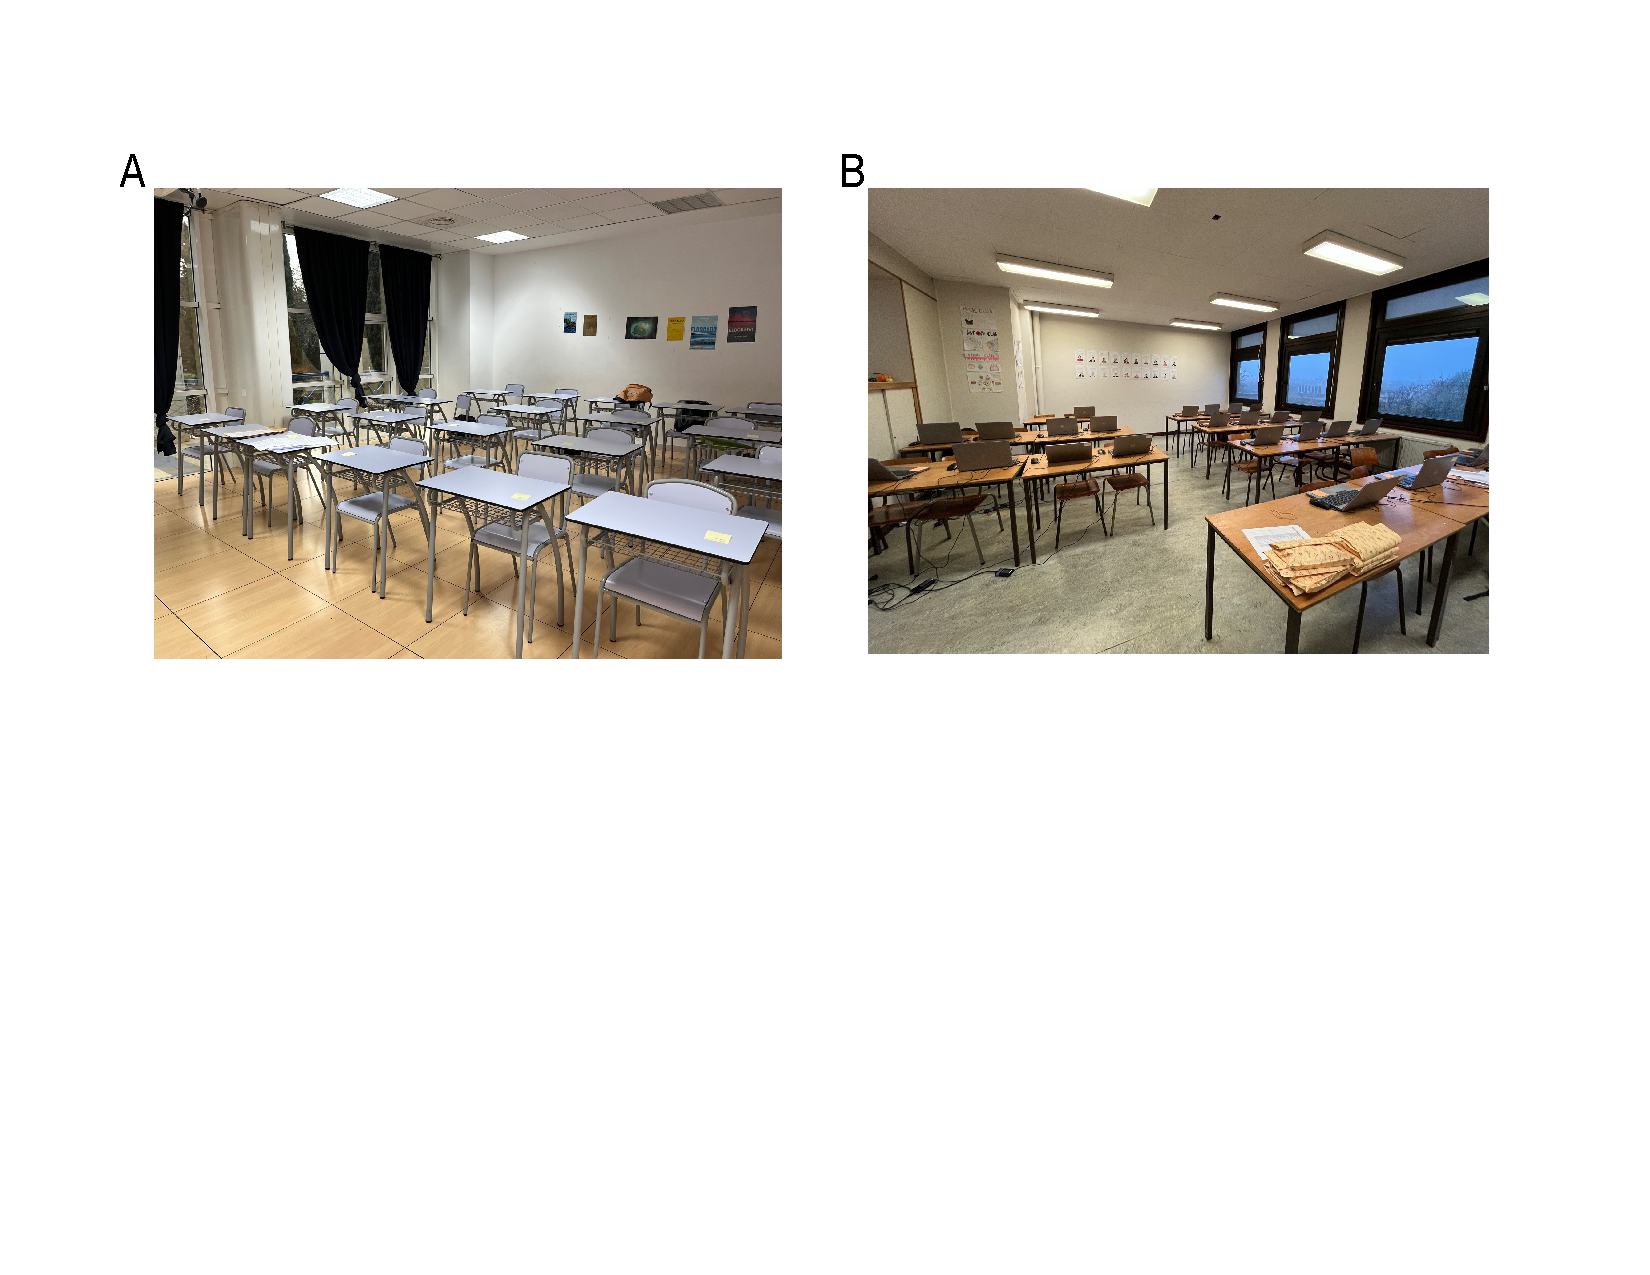
\includegraphics[keepaspectratio]{assets/pictures/classrooms.pdf}}
\caption{Classrooms used for the experiment in Seville (\textbf{A}) and in Brussels (\textbf{B}).}\label{fig:classrooms}
\end{figure}

\subsection{Experimental sessions}\label{experimental-sessions}

About ten experimental sessions were conducted at the schools between November 11 and 12, 2023, in Brussels and February 8 and 9, 2024, in Seville. Each session took about two hours. In the first 45-60 minutes, students received a personal computer and were asked to perform multiple tasks online using the AI tutor, including answering a questionnaire. In the following 45-60, there was a group discussion on how the students found the interactions with the AI tutor and a more general debate on how they perceived the potential benefits and drawbacks of integrating LLMs in the classroom. The results of the group discussions are not discussed in this paper; however, they were used as material for interpreting the results of the experimental study.

\subsection{Experimental Conditions}\label{experimental-conditions}

Figure \ref{fig:design} illustrates the two randomised manipulations in our experimental design: (1) AI step-by-step reasoning and (2) Socratic vs non-Socratic AI.

\begin{figure}
\centering
\pandocbounded{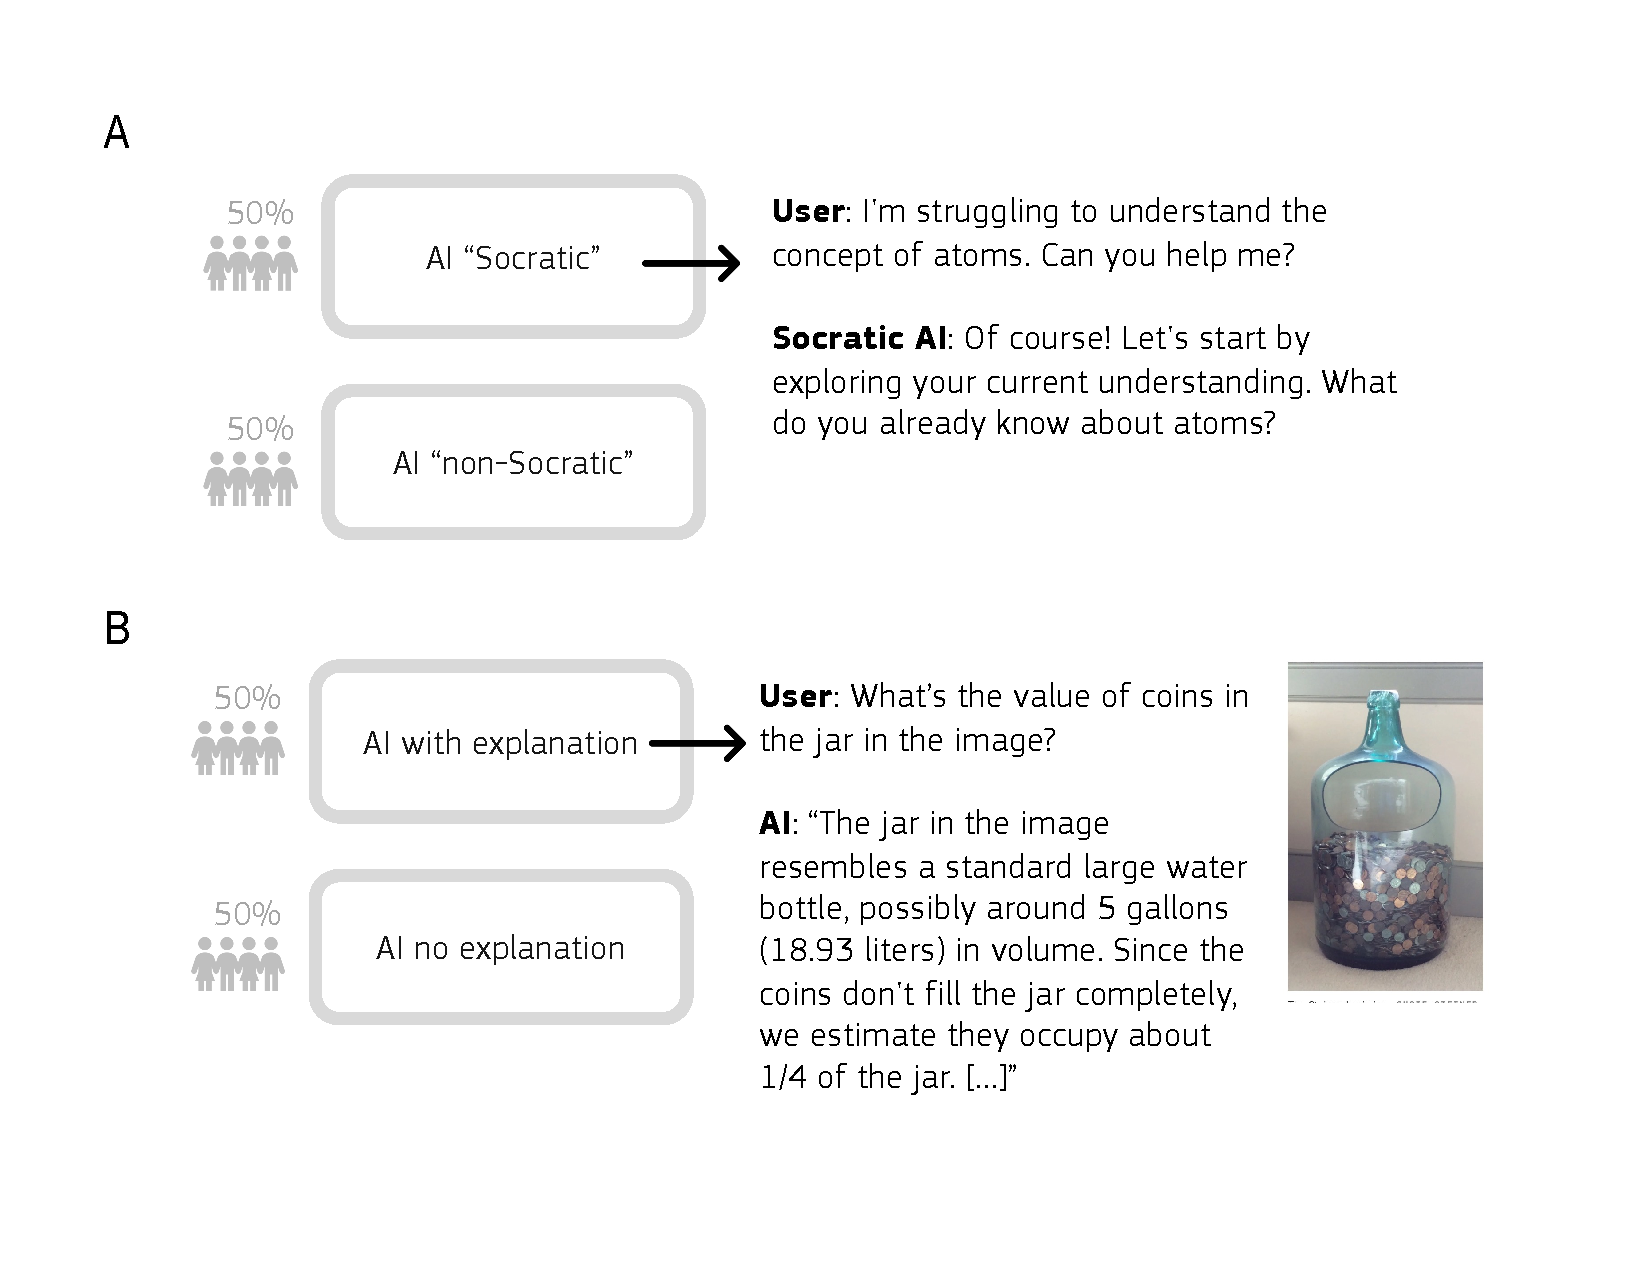
\includegraphics[keepaspectratio]{assets/pictures/experimental_design.pdf}}
\caption{The experimental design involves two manipulations: \textbf{A.} Socratic vs Non-Socratic; \textbf{B.} AI solution with explanation vs AI solution (without explanation)}\label{fig:design}
\end{figure}

\paragraph*{AI step-by-step reasoning}\label{ai-step-by-step-reasoning}
\addcontentsline{toc}{paragraph}{AI step-by-step reasoning}

The first manipulation focuses on a task in which students are asked to estimate the value of coins in a jar (see Section \ref{sec:si-ai-explanation} for the details).\footnote{This is a common experimental activity in economics, especially in the context of auction theory (\citeproc{ref-thaler1988anomalies}{Thaler 1988}). The task is ideal in our setting because it requires participants to guess based on limited information, thus creating a situation where AI-generated assistance could potentially influence their decisions.} Specifically, we used the coin jar from Steiner's experiment (\citeproc{ref-steiner2015turns}{Steiner 2015}), aimed originally at assessing Internet users' guessing accuracy. For this intervention, we varied the AI's response by providing either a complete answer, which included both an estimated value and a step-by-step explanation generated by the AI tutor, or a partial answer that provided only the estimate without additional details. In both conditions, all participants received the same estimated value (\$213), but those in the full-answer condition also viewed an explanation outlining the step-by-step reasoning the AI used to arrive at this estimation based on the jar image.\footnote{Using GPT 4.0, we uploaded the image of the coin jar asking for an estimate of the value of coins for ten times. We then selected the median response for the experiment.}

This setup allows us to examine how AI-provided explanations affect students' performance and their perceptions of the AI's accuracy. Specifically, we focus on three outcome variables: (1) the propensity to update their initial guess and size of their updates, (2) the accuracy of students' final estimations, measured as the (absolute) difference between their guesses and the actual coin value, and (3) students' perceived accuracy of the AI, rated on a scale from low to high. We also asked participants (4) to rate the perceived accuracy of the mean guess among 600 people (\$596), which exaggerated the correct value, as reported in the original article (\citeproc{ref-steiner2015turns}{Steiner 2015}).

\paragraph*{Socratic vs Non-Socratic AI}\label{socratic-vs-non-socratic-ai}
\addcontentsline{toc}{paragraph}{Socratic vs Non-Socratic AI}

The second manipulation involved randomly assigning students to one of two different types of AI tutors: Socratic or non-Socratic AI tutors. Both tutors were powered by the same underlying large language model (GPT-4). Still, each was instructed with different ``system messages'' to create different behaviours, as illustrated in Table \ref{tab:prompts}.\footnote{An AI's system message guides how the AI interprets the conversations by setting paramters for interaction.} For the Socratic tutor, the system message asked the model to engage students with open-ended, thought-provoking questions, encouraging them to think critically about their responses. In contrast, the non-Socratic AI tutor was instructed to provide concise, direct answers without necessarily engaging in deeper dialogue or posing further questions.

\begin{table}

\caption{\label{tab:prompts}Prompt instructions associated with the AI Tutor's treatments}
\centering
\begin{tabular}[t]{l>{\raggedright\arraybackslash}p{4in}}
\toprule
AI.Tutor & Prompt.instruction\\
\midrule
Socratic & You are a Socratic tutor. You always answer using the Socratic style, asking just the right questions to help students learn to think for themselves, breaking down the problem into simpler parts until it's at the right level for them. You provide concise information and explanations understandable for 8th to 10th grade students.\\
Non-Socratic & You are a didactic tutor. You provide concise information and explanations understandable for 8th to 10th grade students.\\
\bottomrule
\end{tabular}
\end{table}

This setup allowed us to investigate the impact of different pedagogical AI tutoring approaches on students' performance and perceptions. Specifically, we asked students to use the AI tutor while performing three tasks: guess an unknown quantity (``How much water in litres do students consume at our school each week?''); express an opinion and write a short essay (``What is your opinion about the effect of social media on teenagers?''); respond to physics questions on how sound propagates in different media (``In which of the following materials does sound travel faster?''). These questions enabled us to assess the AI tutor's impact on students' learning and problem-solving abilities.

We focused on two primary metrics: (1) confidence in their answers, (2) perceived usefulness of interacting with the AI tutor. Specifically, students were asked, ``How confident are you that the answer you provided is accurate?'' on a five-point scale ranging from ``not confident at all'' to ``very confident.'' They were also asked ``How helpful was it to interact with the AI tutor?'' This was also rated on a five-point scale, from ``Not at all helpful'' to ``Very helpful.'' Only for task 3, we had an additional metric which was the correctness of their answers.

\subsection{Background Measures}\label{background-measures}

As an initial step in our analysis, and to better understand students' awareness of and attitudes toward AI, we developed a brief four-question ``AI in Education Attitudes Scale.'' This scale was adapted from the broader AI Attitudes Scale proposed by Schepman and Rodway (\citeproc{ref-schepman2020initial}{Schepman and Rodway 2020}). These questions included: Do you agree or disagree that society will benefit from a future of AI? Do you agree or disagree that AI is dangerous? Do you agree or disagree that AI will foster students' learning in the future? Do you agree or disagree that AI is often misused by students?

Finally, to consider participants' academic performance and skills, participants were also asked about their school grades and how often they complete their homework assignments on time and what factors affect their ability to do so. Self-reported experience using ChatGPT (the main LLM available at the time of the study) was also asked, including a question on their estimation of how many of their peers use ChatGPT for their homework.

Section \ref{sec:questionnaire} presents the complete questionnaire.

\section{Results}\label{sec:results}

\subsection{Overview of Student Demographics}\label{overview-of-student-demographics}

A total of 122 students participated in the study, 64 in Brussels and 58 in Seville. The sample was gender balanced. Over half of the students reported B+ grades and prior use of ChatGPT, with boys more likely to report ChatGPT experience. Around 50\% reported to always complete homework on time, with a minority reporting less than always, with factors like time management (17\% in Brussels, 25\% in Seville) and material comprehension (56\% in Brussels, 28\% in Seville) affecting completion. Students' self-efficacy varied by task, with 30\% of the students feeling they could ``easily'' write a technology essay (task 2) but only 6\% and 11\% feeling confident about explaining sound propagation (task 3) or solving a numerical estimation task such as guessing the litres of water in a pool (task 1). Thus, the sample was substantially homogeneous in terms of demographics but diverse in terms of self-efficacy.

Table \ref{tab:summary-statistics} illustrates the distribution of student characteristics according to the treatment assignment for the Socratic versus Non-Socratic AI tutor. (A similar table for the AI step-by-step reasoning assignment can be shown.) The sample characteristics were generally balanced across treatments. Only one out of ten associations with the treatment assignment was statistically significant for the Socratic/Non-Socratic conditions, and no significant associations were found for the AI Step-by-step reasoning assignment. Thus, only one out of twenty Fisher's exact tests showed a significant result (p \textless{} 0.05), indicating a good balance across treatments.

\begin{table}
\centering
\caption{\label{tab:summary-statistics}Sample characteristics}
\centering
\begin{tabular}[t]{llrrr}
\toprule
Name & Value & \% Non-Socratic & \% Socratic & N\\
\midrule\arrayrulecolor{gray!20}
Gender & Boy & 47.5 & 54.8 & 62\\
\hline
 & Girl & 52.5 & 45.2 & 59\\
\hline
Grades & Average or lower grades & 44.8 & 46.8 & 55\\
\hline
 & Top grades & 55.2 & 53.2 & 65\\
\hline
Has used ChatGPT & No & 37.3 & 42.9 & 49\\
\hline
 & Yes & 62.7 & 57.1 & 73\\
\hline
Homework difficulties & Clear instructions from teachers & 20.3 & 9.7 & 18\\
\hline
 & Effective time management & 11.9 & 29.0 & 25\\
\hline
 & Lack of distractions & 10.2 & 17.7 & 17\\
\hline
 & Support from family or peers & 6.8 & 8.1 & 9\\
\hline
 & Understanding the material & 50.8 & 35.5 & 52\\
\hline
Homework on time & Always on time & 55.9 & 41.9 & 59\\
\hline
 & Sometimes or rarely on time & 6.8 & 8.1 & 9\\
\hline
 & Usually on time & 37.3 & 50.0 & 53\\
\hline
Homework weekly study & 0-1 hours & 40.7 & 46.8 & 53\\
\hline
 & 1-2 hours & 44.1 & 33.9 & 47\\
\hline
 & 2+ hours & 15.3 & 19.4 & 21\\
\hline
Location & Brussels & 55.9 & 49.2 & 64\\
\hline
 & Seville & 44.1 & 50.8 & 58\\
\hline
Self-efficacy (essay) & Could do easily & 32.2 & 38.1 & 43\\
\hline
 & Could do with a bit of effort & 52.5 & 52.4 & 64\\
\hline
 & I couldn't do this on my own & 3.4 & 3.2 & 4\\
\hline
 & I would struggle on my own & 11.9 & 6.3 & 11\\
\hline
Self-efficacy (guess) & Could do easily & 11.9 & 14.3 & 16\\
\hline
 & Could do with a bit of effort & 33.9 & 27.0 & 37\\
\hline
 & I couldn't do this on my own & 15.3 & 23.8 & 24\\
\hline
 & I would struggle on my own & 39.0 & 34.9 & 45\\
\hline
Self-efficacy (sound) & Could do easily & 6.8 & 6.3 & 8\\
\hline
 & Could do with a bit of effort & 30.5 & 46.0 & 47\\
\hline
 & I couldn't do this on my own & 16.9 & 14.3 & 19\\
\hline
 & I would struggle on my own & 45.8 & 33.3 & 48\\
\arrayrulecolor{black}\bottomrule
\end{tabular}
\end{table}

\subsection{Attitudes Towards AI}\label{attitudes-towards-ai}

As illustrated in Figure \ref{fig:attitudes-AI}, students expressed conflicting views on the role of AI in education. On the one hand, a majority felt that AI is often misused by students (65\%) and potentially dangerous (57\%). On the other hand, most students also anticipated that AI would enhance student learning in the future (59\%) and contribute positively to society (65\%). These findings suggest that most students in our sample are aware of the risks of misuse and safety with a prevailing optimism that AI could support educational growth and societal progress.

\begin{figure}
\centering
\pandocbounded{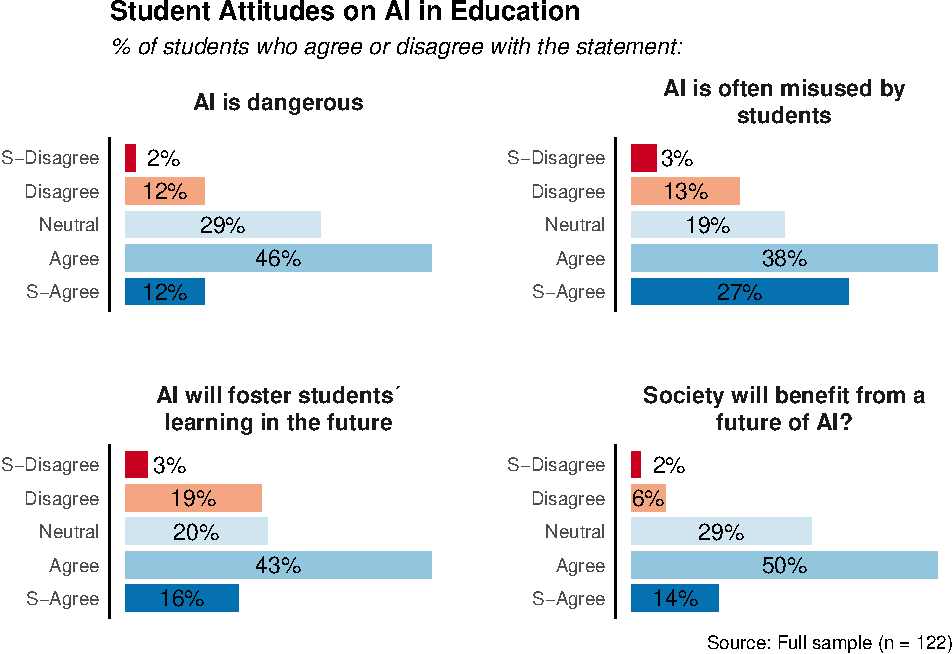
\includegraphics[keepaspectratio]{main_report_files/figure-latex/attitudes-AI-1.pdf}}
\caption{\label{fig:attitudes-AI}Student attitudes on AI in education}
\end{figure}

\subsection{The Impact of AI Step-by-step Reasoning Exposure}\label{the-impact-of-ai-step-by-step-reasoning-exposure}

We tested whether showing students AI-generated step-by-step reasoning affected how they used the AI's prediction, compared to just seeing the prediction without any reasoning. We measured students' accuracy using the absolute difference between each student \(i\)'s prediction and the actual value of coins:
\[
  \text{absolute error}_i = |\text{guess}_i - \text{actual value}|,
\]
for \(i =1, \cdots, N\), where a smaller absolute error indicated greater accuracy.

The absolute error distribution in our sample was positively skewed, complicating the testing for mean differences. Consequently, we shifted our analysis towards treatment differences in the median absolute error, as illustrated in Figure \ref{fig:boot-accuracy}. We applied bootstrap resampling to estimate the median difference across treatment groups and the corresponding confidence intervals.\footnote{Outliers were detected in the data and removed from the bootstrap analysis. One student provided a notably high guess of 6969. However, this value deviated substantially from both the overall distribution and the student's initial guess, suggesting an error rather than an informed estimate.} Results indicated that, although both groups received the same exact AI estimate of \$213, students who also received AI-generated step-by-step reasoning demonstrated a significantly higher accuracy, reflected by a lower median of the absolute error (p = 0.08). This evidence indicates that exposure to AI reasoning contributed to an improvement in student performance.

\begin{figure}
\centering
\pandocbounded{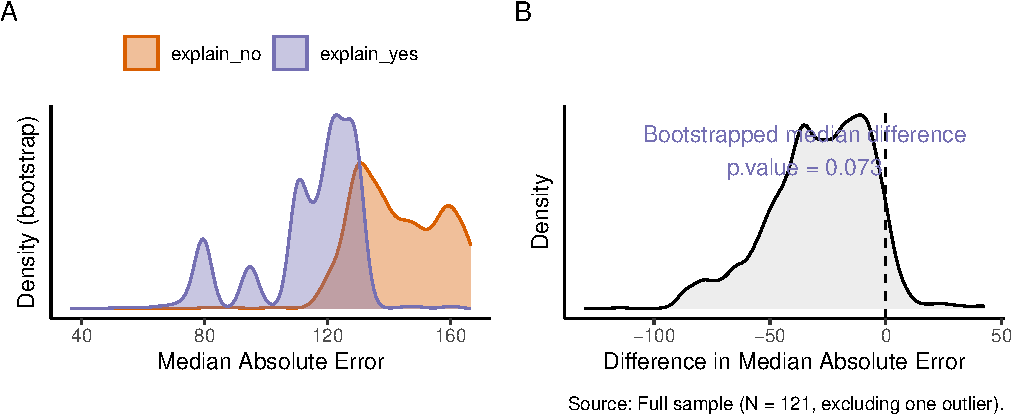
\includegraphics[keepaspectratio]{main_report_files/figure-latex/boot-accuracy-1.pdf}}
\caption{\label{fig:boot-accuracy}Comparison of Students' Absolute Error in Estimating Coin Jar Value with and without AI Explanations. All students received the AI-generated estimate of \$213 (the correct value was \$379.54). Still, those in the AI reasoning treatment also viewed the AI-generated step-by-step explanation for the estimation. Exposure to the AI-generated explanation significantly reduced the students' median absolute error.}
\end{figure}

We subsequently examined students' perceptions of the AI's prediction accuracy on a five-point rating. We noticed that 53\% of students who did not receive step-by-step reasoning considered the AI estimate as either ``good'' (39\%) or ``very good'' (14\%) compared to 43\% of students exposed to the AI reasoning (19\% and 24\%, respectively). This gap of ten percentage points suggests that students viewed the AI as more accurate when the AI-generated guess was presented as a ``black box.'' However, we didn't have enough observations to reach a statistically significant association (Fisher's test, p = .27), and even regression analysis, controlling for individual characteristics, showed no significant association (Figure \ref{fig:perceived-accuracy-coins}).

Conversely, exposure to the AI step-by-step reasoning significantly influenced students' perceptions of the ``human'' estimate of \$596. This value was the average guess of 600 participants in the initial study (\citeproc{ref-steiner2015turns}{Steiner 2015}), which exceeded the correct value (\$379.54) by about the same amount as the AI guess underestimated it (\$213). Notably, all groups received the same human and AI estimates, but while 64\% of students in the control group rated the human estimate as ``poor'' or ``very poor,'' only 45\% of students exposed to AI reasoning did so. Although this difference was marginally significant (Fisher's exact test, p = 0.15), regression analysis, controlling for student's location, gender, their initial estimate of the value of coins, and experience with ChatGPT, confirmed that AI exposure led students to rate the human estimate about half a point more favourably (p \textless{} 0.05), as shown in Figure \ref{fig:perceived-accuracy-coins}. This finding underscores the complex relationship between AI and learning. It suggests that students exposed to the AI's step-by-step reasoning may have identified minor errors, thus increasing their expectations of human accuracy, and those who viewed AI as a ``black box'' tended to underrate human estimates.

\begin{figure}
\centering
\pandocbounded{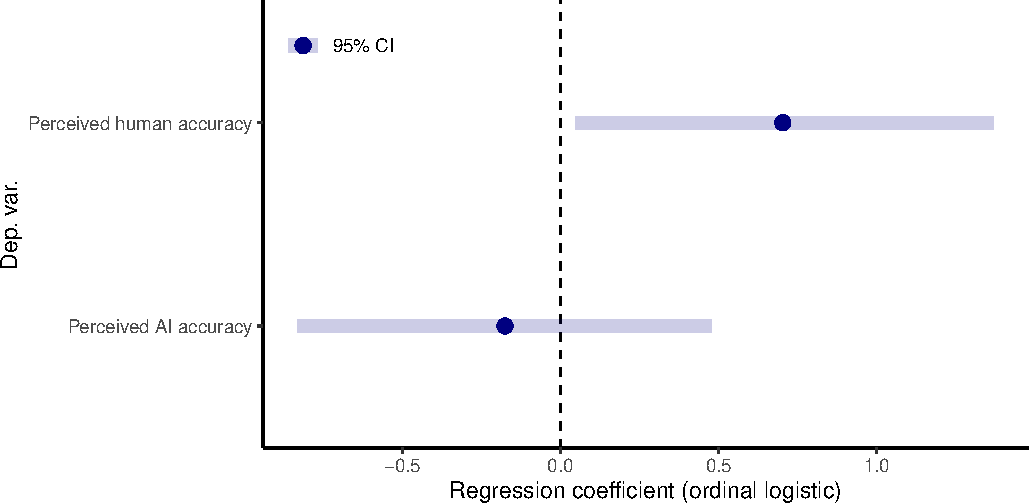
\includegraphics[keepaspectratio]{main_report_files/figure-latex/perceived-accuracy-coins-1.pdf}}
\caption{\label{fig:perceived-accuracy-coins}Comparison of students' perceived accuracy of AI and human estimates across treatments on a five-point scale. Coefficients from separate ordinal logistic regressions controlling for students' location, gender, and prior experience with ChatGPT. Positive coefficients indicate increased perceived accuracy associated with students' exposure to AI reasoning.}
\end{figure}

\subsection{A Comparison of Socratic vs Non-Socratic AI}\label{a-comparison-of-socratic-vs-non-socratic-ai}

\paragraph*{Student-AI Interactions}\label{student-ai-interactions}
\addcontentsline{toc}{paragraph}{Student-AI Interactions}

Figure \ref{fig:messages} shows the students' message length and frequency in the Socratic AI and Non-Socratic AI groups, allowing us to compare the student-AI interactions across treatment groups. As shown in the figure, Socratic AI students exchanged a median of 20 messages, significantly more than the eight messages by non-Socratic AI students (Wilcoxon test, p \textless{} 0.01). In addition, the Socratic AI's messages were significantly shorter, with a median of 42 words, compared to 123 for the non-Socratic tutor (Wilcoxon test, p \textless{} 0.01). Socratic students also used fewer words, with two peaks: one at ten and the other at one word. This evidence supports the hypothesis that the Socratic tutor encouraged more engagement and interaction, resembling a relatively more genuine student-tutor talk.

\begin{figure}
\centering
\pandocbounded{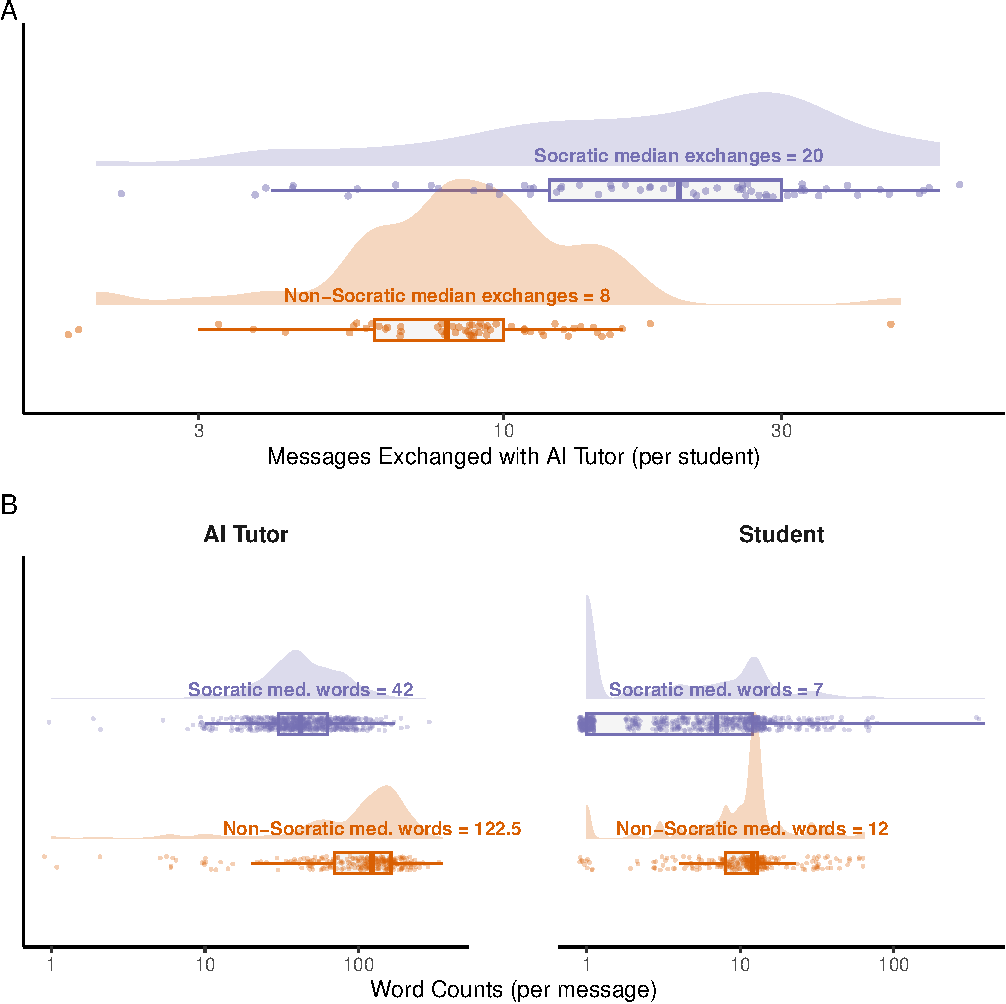
\includegraphics[keepaspectratio]{main_report_files/figure-latex/messages-1.pdf}}
\caption{\label{fig:messages}Comparison of message frequency and word count per message across Socratic and non-Socratic treatments. Top panel (\textbf{A}) shows differences in the frequency of messages exchanged, while the bottom panels (\textbf{B} ) depict the word counts per message for the AI tutor (left) and the students (right).}
\end{figure}

\paragraph*{Students' Confidence in Their Responses}\label{students-confidence-in-their-responses}
\addcontentsline{toc}{paragraph}{Students' Confidence in Their Responses}

We hypothesised Socratic AI would promote a deeper understanding of the task, raising students' confidence in their answers. To test this hypothesis, we examined students' self-reported confidence using a five-point scale at the end of each task. As shown in Figure \ref{fig:confidence}, the differences in confidence levels between the treatment groups were minimal. Among Socratic students, 25\% reported feeling ``very confident,'' and 33\% felt ``confident'' compared to 21\% and 38\% among non-Socratic students. These differences were not statistically significant, even with regression analysis controlling for student-task differences (Figure \ref{fig:confidence-regression}). Thus, our analysis found no evidence of treatment effects on students' confidence levels.

\begin{figure}
\centering
\pandocbounded{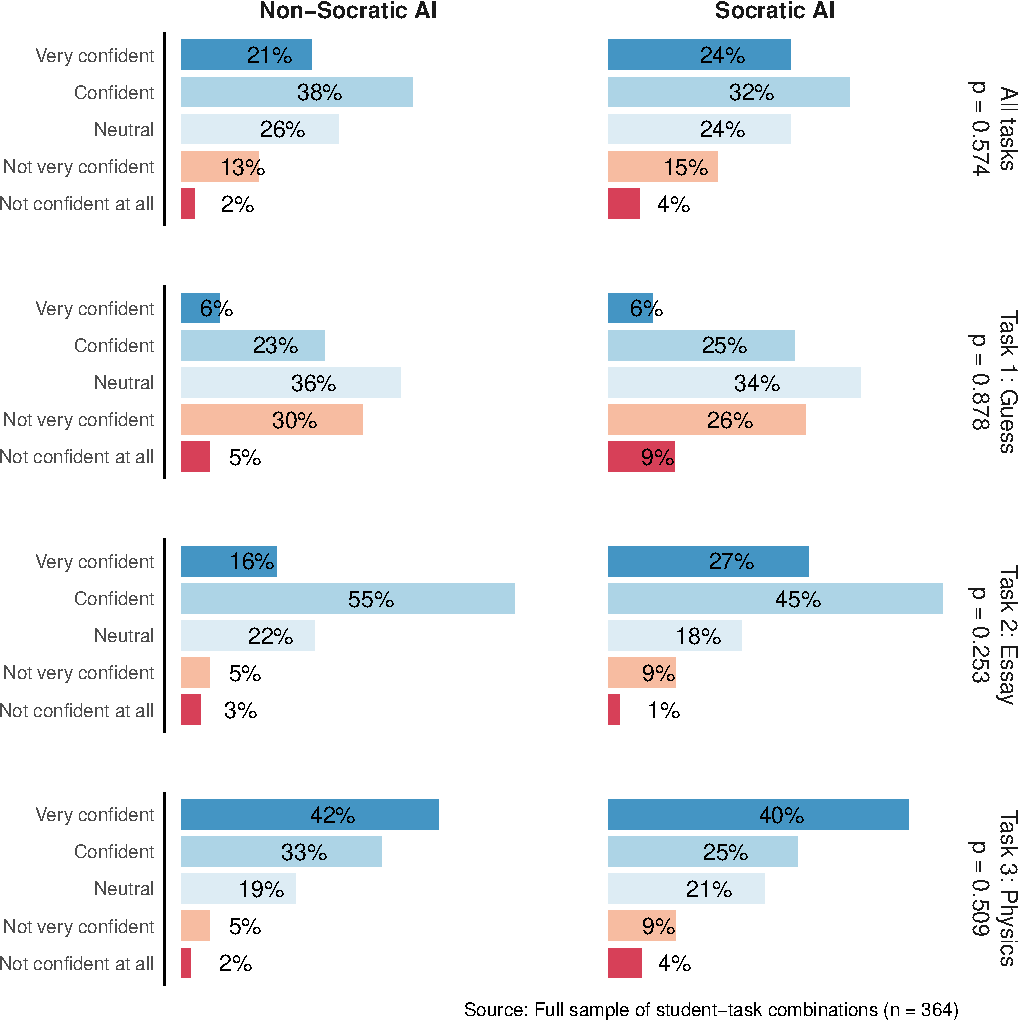
\includegraphics[keepaspectratio]{main_report_files/figure-latex/confidence-1.pdf}}
\caption{\label{fig:confidence}This figure shows the impact of Socratic AI on students' confidence levels in their performance across three different tasks. Despite some differences between the Socratic and Non-Socratic groups, we found no significant association between the treatment assignment and students' declared confidence levels.}
\end{figure}

\begin{figure}
\centering
\pandocbounded{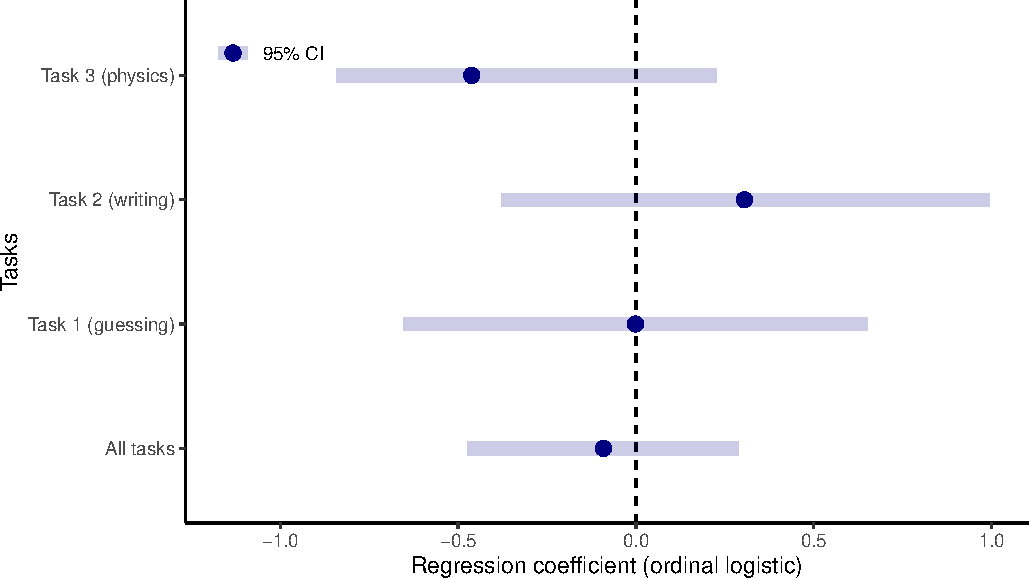
\includegraphics[keepaspectratio]{main_report_files/figure-latex/confidence-regression-1.pdf}}
\caption{\label{fig:confidence-regression}This figure shows the coefficients from separate ordinal logistic regressions on students' confidence in their answer on a five-point scale, controlling for students' self-efficacy per task and task fixed effect. Results show no significant association between the treatment assignment and students' confidence levels.}
\end{figure}

Further explorative regression analysis to examine potential treatment interactions shows that Socratic AI students with prior ChatGPT experience reported significantly less confidence (p \textless{} 0.1) than Non-Socratic AI students. This explorative finding suggests that experienced users may perceive new or unconventional AI tutoring methods as less effective or even counterproductive, indicating that encouraging the use of such AI tutoring tools among experienced ChatGPT students can be challenging.

\paragraph*{Perceived Helpfulness of AI Tutor}\label{perceived-helpfulness-of-ai-tutor}
\addcontentsline{toc}{paragraph}{Perceived Helpfulness of AI Tutor}

We examined differences in students' perceptions of the AI tutor's helpfulness (How helpful was it to interact with the AI tutor?) on a five-point scale, from ``Not at all helpful'' to ``Very helpful.''\footnote{Due to a coding issue, the scale used in Brussels and Seville differed slightly in the labels: Seville's students saw ``Extremely helpful'' whereas Brussels students saw ``Very helpful.'' However, this issue has a minimal impact on the overall results, as results focus on the negative labels (``not at all helpful'' or ``not helpful'') and they remain the same even after controlling for location effects in a regression. Additionally, open discussions held with students after the experimental session confirmed that they found the Socratic AI less helpful. This feedback, combined with the observed differences in negative labels, reinforces that the coding discrepancy has a minimal impact on the overall findings.}

In both treatment groups, many students found interacting with the AI tutor ``very helpful'' or ``helpful'', with 56\% of the non-Socratic and 44\% of the Socratic students, as shown in Figure \ref{fig:helpfulness}. However, the Socratic treatment group showed a bimodal distribution, with a substantial fraction of students (21\%) finding the interaction ``not at all helpful.'' The association between perceived helpfulness and treatment assignment was statistically significant (Fisher's exact test, p = 0.025), providing evidence that Socratic AI was less helpful to certain students. This association, however, was stronger for Task 1 and Taks 3 than Task 2, suggesting an association between the perceived AI's helpfulness and the type of task. Ordinal logistic regression accounting for individual student and task characteristics, including self-efficacy per task, revealed a statistically significant negative difference that corresponds to a drop of approximately 13 percentage points in perceived helpfulness associated with the Socratic AI, as illustrated in Figure \ref{fig:helpful-regression}. See Section \ref{sec:regress-confidence} for more details.

\begin{figure}
\centering
\pandocbounded{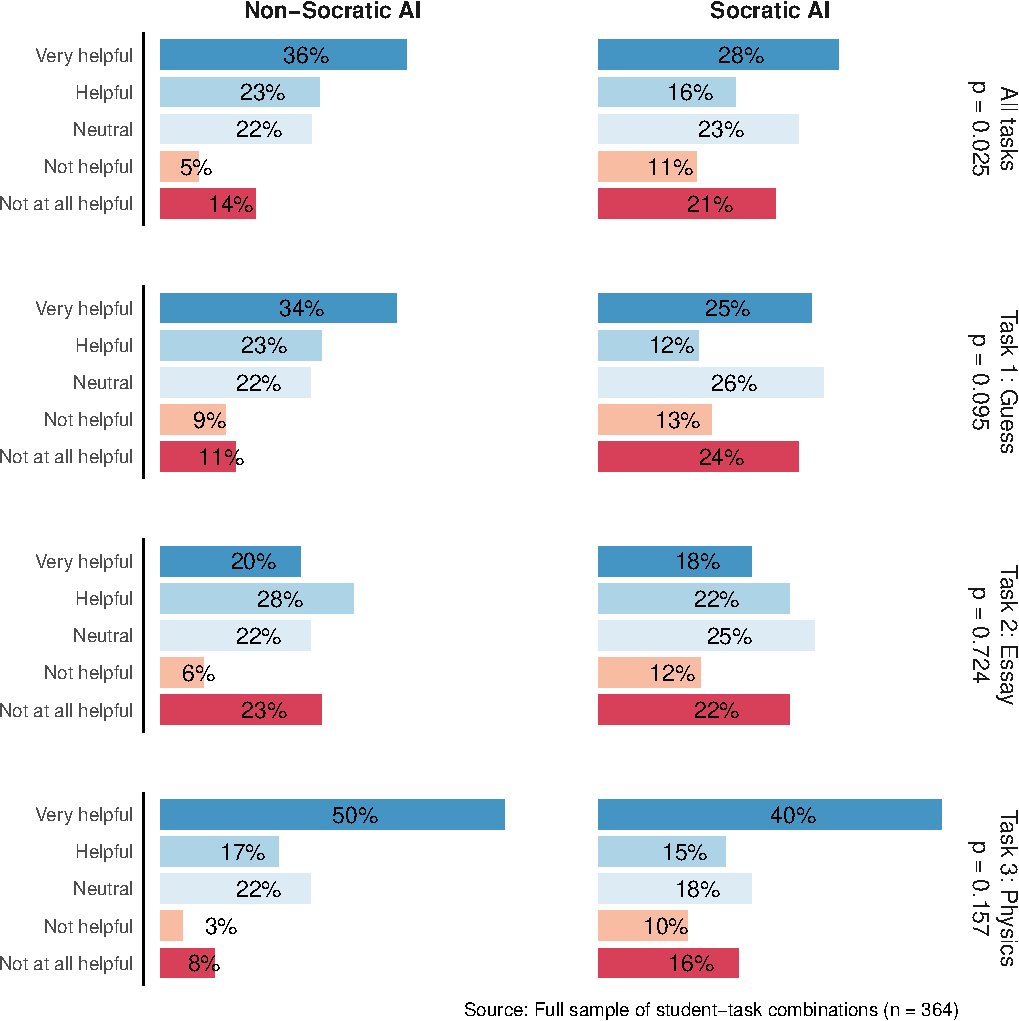
\includegraphics[keepaspectratio]{main_report_files/figure-latex/helpfulness-1.pdf}}
\caption{\label{fig:helpfulness}This figure shows the impact of Socratic AI on students' perceived helpfulness of the AI tutor across three different tasks.}
\end{figure}

\begin{figure}
\centering
\pandocbounded{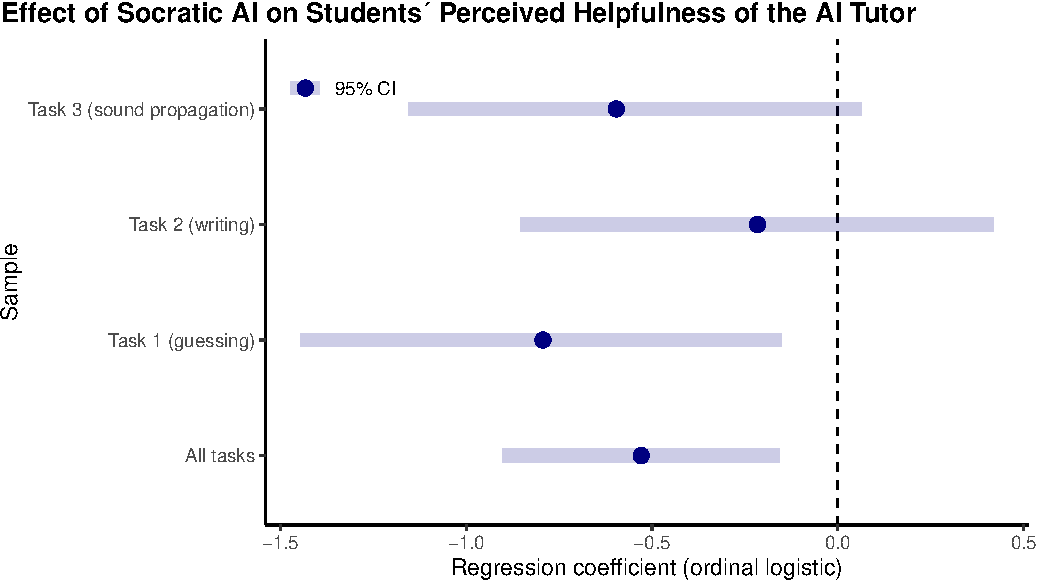
\includegraphics[keepaspectratio]{main_report_files/figure-latex/helpful-regression-1.pdf}}
\caption{\label{fig:helpful-regression}The impact of Socratic AI on students' confidence levels in their performance across three different tasks. Despite some differences between the Socratic and Non-Socratic groups, we found no significant association between the treatment assignment and students' declared confidence levels}
\end{figure}

\paragraph*{Learning Outcomes and Knowledge Retention}\label{learning-outcomes-and-knowledge-retention}
\addcontentsline{toc}{paragraph}{Learning Outcomes and Knowledge Retention}

To evaluate the impact of learning, we compared the correctness of responses to Task 3, which focused on sound propagation, and assessed knowledge retention using a follow-up question on the same topic without AI assistance. As shown in Figure \ref{fig:learning}, the use of AI significantly enhanced students' response accuracy. Before interacting with the AI tutor, only 32\% of students correctly answered that sound travels faster in water than air due to water's higher density. After AI interaction, this percentage nearly doubled increasing to 68\%. However, there was no significant difference in learning outcomes between the Socratic and non-Socratic AI approaches, as illustrated in the figure. Moreover, when presented with a follow-up question (asking in which medium sound travels fastest among gold, rubber, warm air, cold air, and water), only 18\% of students responded correctly by selecting the denser material (i.e., gold), again with no significant difference across treatments. This result suggests two implications. Firstly, we found no evidence of Socratic AI improving learning. Secondly, our results confirmed a problem of limited retention of the insights obtained with AI assistance or difficulty in applying such learning to novel scenarios.

\begin{longtable}[]{@{}
  >{\raggedright\arraybackslash}p{(\linewidth - 6\tabcolsep) * \real{0.5698}}
  >{\raggedleft\arraybackslash}p{(\linewidth - 6\tabcolsep) * \real{0.1395}}
  >{\raggedleft\arraybackslash}p{(\linewidth - 6\tabcolsep) * \real{0.1512}}
  >{\raggedleft\arraybackslash}p{(\linewidth - 6\tabcolsep) * \real{0.1395}}@{}}
\caption{\label{tab:learning}\% of students in each treatment group by responses to the question `Does sound travel faster in water than air?'}\tabularnewline
\toprule\noalign{}
\begin{minipage}[b]{\linewidth}\raggedright
\end{minipage} & \begin{minipage}[b]{\linewidth}\raggedleft
Full sample
\end{minipage} & \begin{minipage}[b]{\linewidth}\raggedleft
Non-Socratic
\end{minipage} & \begin{minipage}[b]{\linewidth}\raggedleft
Socratic AI
\end{minipage} \\
\midrule\noalign{}
\endfirsthead
\toprule\noalign{}
\begin{minipage}[b]{\linewidth}\raggedright
\end{minipage} & \begin{minipage}[b]{\linewidth}\raggedleft
Full sample
\end{minipage} & \begin{minipage}[b]{\linewidth}\raggedleft
Non-Socratic
\end{minipage} & \begin{minipage}[b]{\linewidth}\raggedleft
Socratic AI
\end{minipage} \\
\midrule\noalign{}
\endhead
\bottomrule\noalign{}
\endlastfoot
Same speed & 9.1 & 6.8 & 11.3 \\
Water is faster because higher density (correct) & 31.4 & 35.6 & 27.4 \\
Water is faster because lower density & 11.6 & 10.2 & 12.9 \\
Water is slower because higher density & 41.3 & 42.4 & 40.3 \\
Water is slower because lower density & 6.6 & 5.1 & 8.1 \\
\end{longtable}

\begin{figure}
\centering
\pandocbounded{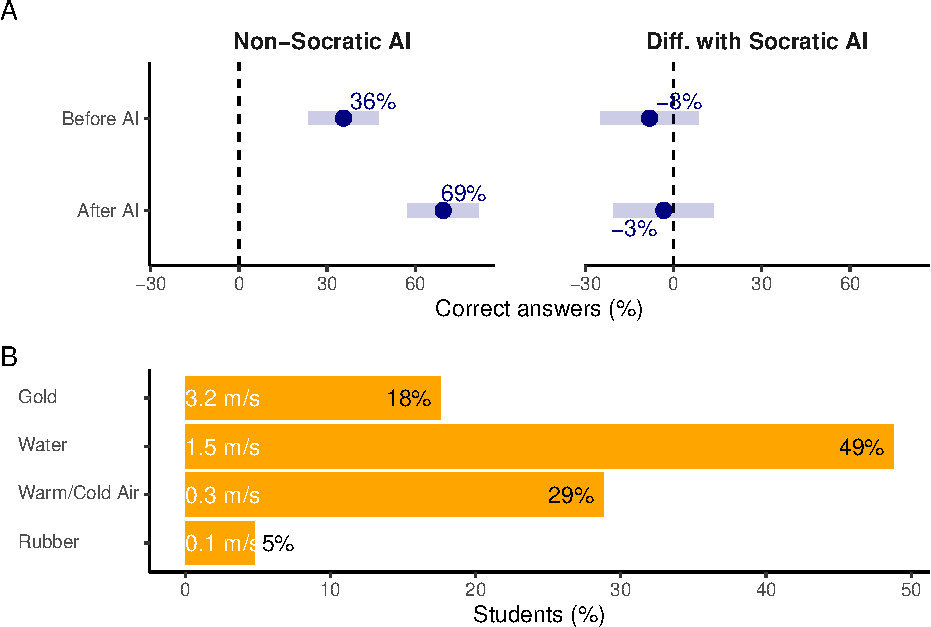
\includegraphics[keepaspectratio]{main_report_files/figure-latex/learning-1.pdf}}
\caption{\label{fig:learning}Effects on learning: \textbf{A} shows the \% of correct responses about the physics of sound propagation, illustrating the positive effect of interacting with the AI tutor, while no differences are associated with the Socratic AI. \textbf{B} shows the results of the verification question asking students to identify the fastest material for sound propagation (speed as meter per second reported) without AI assistance. Only 18\% responded accurately, indicating limited learning.}
\end{figure}

\section{Discussion}\label{discussion}

The current results indicate several important implications. First, we found that students significantly benefit from AI-generated step-by-step reasoning accompanying solutions, mainly when performing open-ended tasks like estimating unknown quantities. This finding aligns with previous research demonstrating that LLMs can enhance student performance and that explanations help children develop critical thinking. However, our results underscore that the key mechanism driving AI improvements is the step-by-step reasoning provided by the AI, which allows students to understand better and engage with problem-solving. This insight suggests that teachers should focus on educating students to enhance their ability to evaluate and judge the correctness of AI-generated reasoning.

Furthermore, our study reveals that step-by-step reasoning not only helps students in solving problems but also enhances students' ability to evaluate AI-generated information critically. This was evidenced by the more positive evaluations of human-generated guesses compared to AI-generated solutions, suggesting that students could better assess and challenge AI predictions. This contribution extends the existing literature by showing that AI can foster critical thinking and analytical skills when coupled with transparent reasoning, instead of being presented as a ``black box.''

In addition, we compared various ways to structure student-AI interactions and, more specifically, the effectiveness of Socratic AI (an interactive, questioning-based AI) with non-Socratic AI. Our results showed that Socratic AI was more engaging and promoted greater interaction, aligning with the notion that AI-student interactions should be dynamic and dialogical. However, contrary to our expectations, we found no significant differences in students' self-reported confidence in the accuracy of their answers or in the correctness of their responses despite the more frequent interactions with the Socratic AI. Additionally, the Socratic AI's perceived helpfulness was rated lower compared to the non-Socratic AI. These results cast some doubts on the effectiveness of Socratic AI in short-term tasks or, more broadly, the effect of certain kinds of AI-student interactions. As such, existing pedagogical practices extensively used in human-human interaction might not always work in human-AI interaction. This underscores that new pedagogical paradigms are needed to integrate AI into pedagogical practices effectively.

Our findings indicate that simply interacting with AI cannot promote meaningful and lasting learning. In our initial test on sound propagation, approximately half of the students could revise their initial answers based on AI interactions, improving their response accuracy from 30\% to 70\%. However, in a verification task where students had no access to AI, the majority failed to identify the correct answer, mistakenly claiming that sound propagates faster in water than in gold. Most students exhibited this misunderstanding, which supports key concerns that AI-generated answers alone may not facilitate effective learning, and that Socratic AI does not mitigate this risk.

Our results suggest that AI has great potential as an educational tool, but its implementation requires careful consideration. First, students with prior experience in using AI tools may not readily adopt new pedagogical approaches, especially if they perceive them as less effective than commercially available alternatives. Second, the effectiveness of the pedagogical approach may vary depending on the nature of the task, complicating the design of a one-size-fits-all solution for AI-assisted learning.

Several limitations of our study should be acknowledged. The small sample size limits the generalizability of our findings, though the controlled environment and the use of multiple tasks help mitigate potential noise in the data. Also, our experiment focused on short-term results. Although short term results are important to foster adoption, it is unclear the effectiveness of AI in the long-term. Finally, we conducted our study with a cohort of students possessing strong English proficiency and a clear understanding of the limitations of AI, which may not be representative of the general student population. Furthermore, the experiment was carried out at school and in a secure and anonymous digital environment, with a robust protocol developed to ensure the safe and ethical handling of AI-based interactions in experimental settings. However, it remains to be seen if the results of our analysis will remain when students use AI in the field.

\subsection{Concluding remarks}\label{concluding-remarks}

While our study focused on comparing a fairly general pedagogical approach---Socratic AI, future research should explore the effectiveness of alternative pedagogical approaches and the scalability of AI tools across diverse educational contexts. Yet, our findings have important implications for designing AI tutors, highlighting the importance of providing transparent AI-generated step-by-step reasoning and the challenges of fostering learning through guided AI-student interactions. Therefore, our study suggests that AI systems must engage students interactively and foster critical thinking and problem-solving skills to maximise their educational value. Future developments should focus on refining the integration of AI-generated reasoning and ensuring that AI tools are adaptable to various learning tasks and students' needs.

\section*{References}\label{references}
\addcontentsline{toc}{section}{References}

\phantomsection\label{refs}
\begin{CSLReferences}{1}{0}
\bibitem[\citeproctext]{ref-cleveland2015beyond}
Cleveland, Julie. 2015. \emph{Beyond Standardization: Fostering Critical Thinking in a Fourth Grade Classroom Through Comprehensive Socratic Circles}. Arizona State University.

\bibitem[\citeproctext]{ref-dai2023can}
Dai, Wei, Jionghao Lin, Hua Jin, Tongguang Li, Yi-Shan Tsai, Dragan Gašević, and Guanliang Chen. 2023. {``Can Large Language Models Provide Feedback to Students? A Case Study on ChatGPT.''} In \emph{2023 IEEE International Conference on Advanced Learning Technologies (ICALT)}, 323--25. IEEE.

\bibitem[\citeproctext]{ref-dalim2022promoting}
Dalim, Siti Fairuz, Aina Sakinah Ishak, and Lina Mursyidah Hamzah. 2022. {``Promoting Students' Critical Thinking Through Socratic Method: The Views and Challenges.''} \emph{Asian Journal of University Education} 18 (4): 1034--47.

\bibitem[\citeproctext]{ref-danovitch2021mind}
Danovitch, Judith H, Candice M Mills, Kaitlin R Sands, and Allison J Williams. 2021. {``Mind the Gap: How Incomplete Explanations Influence Children's Interest and Learning Behaviors.''} \emph{Cognitive Psychology} 130: 101421.

\bibitem[\citeproctext]{ref-dejong1986explanation}
DeJong, Gerald, and Raymond Mooney. 1986. {``Explanation-Based Learning: An Alternative View.''} \emph{Machine Learning} 1: 145--76.

\bibitem[\citeproctext]{ref-derakhshan2024chatgpt}
Derakhshan, Ali, and Farhad Ghiasvand. 2024. {``Is ChatGPT an Evil or an Angel for Second Language Education and Research? A Phenomenographic Study of Research-Active EFL Teachers' Perceptions.''} \emph{International Journal of Applied Linguistics}.

\bibitem[\citeproctext]{ref-eke2023chatgpt}
Eke, Damian Okaibedi. 2023. {``ChatGPT and the Rise of Generative AI: Threat to Academic Integrity?''} \emph{Journal of Responsible Technology} 13: 100060.

\bibitem[\citeproctext]{ref-gabriel2020artificial}
Gabriel, Iason. 2020. {``Artificial Intelligence, Values, and Alignment.''} \emph{Minds and Machines} 30 (3): 411--37.

\bibitem[\citeproctext]{ref-gavsevic2023empowering}
Gašević, Dragan, George Siemens, and Shazia Sadiq. 2023. {``Empowering Learners for the Age of Artificial Intelligence.''} \emph{Computers and Education: Artificial Intelligence}. Elsevier.

\bibitem[\citeproctext]{ref-hendrycks2021measuring}
Hendrycks, Dan, Collin Burns, Saurav Kadavath, Akul Arora, Steven Basart, Eric Tang, Dawn Song, and Jacob Steinhardt. 2021. {``Measuring Mathematical Problem Solving with the Math Dataset.''} \emph{arXiv Preprint arXiv:2103.03874}.

\bibitem[\citeproctext]{ref-henkel2024can}
Henkel, Owen, Libby Hills, Adam Boxer, Bill Roberts, and Zach Levonian. 2024. {``Can Large Language Models Make the Grade? An Empirical Study Evaluating Llms Ability to Mark Short Answer Questions in k-12 Education.''} In \emph{Proceedings of the Eleventh ACM Conference on Learning@ Scale}, 300--304.

\bibitem[\citeproctext]{ref-joksimovic2023opportunities}
Joksimovic, Srecko, Dirk Ifenthaler, Rebecca Marrone, Maarten De Laat, and George Siemens. 2023. {``Opportunities of Artificial Intelligence for Supporting Complex Problem-Solving: Findings from a Scoping Review.''} \emph{Computers and Education: Artificial Intelligence} 4: 100138.

\bibitem[\citeproctext]{ref-kalyan2021how}
Kalyan, Ashwin, Abhinav Kumar, Arjun Chandrasekaran, Ashish Sabharwal, and Peter Clark. 2021. {``How Much Coffee Was Consumed During EMNLP 2019? Fermi Problems: A New Reasoning Challenge for AI,''} October. \url{https://arxiv.org/pdf/2110.14207.pdf}.

\bibitem[\citeproctext]{ref-kaplan2023generative}
Kaplan-Rakowski, Regina, Kimberly Grotewold, Peggy Hartwick, and Kevin Papin. 2023. {``Generative AI and Teachers' Perspectives on Its Implementation in Education.''} \emph{Journal of Interactive Learning Research} 34 (2): 313--38.

\bibitem[\citeproctext]{ref-kasneci2023chatgpt}
Kasneci, Enkelejda, Kathrin Seßler, Stefan Küchemann, Maria Bannert, Daryna Dementieva, Frank Fischer, Urs Gasser, et al. 2023. {``ChatGPT for Good? On Opportunities and Challenges of Large Language Models for Education.''} \emph{Learning and Individual Differences} 103: 102274.

\bibitem[\citeproctext]{ref-lam2011socratic}
Lam, Faith. 2011. {``The Socratic Method as an Approach to Learning and Its Benefits.''}

\bibitem[\citeproctext]{ref-lara2020artificial}
Lara, Francisco, and Jan Deckers. 2020. {``Artificial Intelligence as a Socratic Assistant for Moral Enhancement.''} \emph{Neuroethics} 13 (3): 275--87.

\bibitem[\citeproctext]{ref-lee2024cheating}
Lee, Victor R, Denise Pope, Sarah Miles, and Rosalı́a C Zárate. 2024. {``Cheating in the Age of Generative AI: A High School Survey Study of Cheating Behaviors Before and After the Release of ChatGPT.''} \emph{Computers and Education: Artificial Intelligence} 7: 100253.

\bibitem[\citeproctext]{ref-legare2014contributions}
Legare, Cristine H. 2014. {``The Contributions of Explanation and Exploration to Children's Scientific Reasoning.''} \emph{Child Development Perspectives} 8 (2): 101--6.

\bibitem[\citeproctext]{ref-li2024explanatory}
Li, Wei, Xiaolin Zhang, Jing Li, Xiao Yang, Dong Li, and Yantong Liu. 2024. {``An Explanatory Study of Factors Influencing Engagement in AI Education at the k-12 Level: An Extension of the Classic TAM Model.''} \emph{Scientific Reports} 14 (1): 13922.

\bibitem[\citeproctext]{ref-roll2016evolution}
Roll, Ido, and Ruth Wylie. 2016. {``Evolution and Revolution in Artificial Intelligence in Education.''} \emph{International Journal of Artificial Intelligence in Education} 26: 582--99.

\bibitem[\citeproctext]{ref-saxton2019analysing}
Saxton, David, Edward Grefenstette, Felix Hill, and Pushmeet Kohli. 2019. {``Analysing Mathematical Reasoning Abilities of Neural Models.''} \emph{arXiv Preprint arXiv:1904.01557}.

\bibitem[\citeproctext]{ref-schepman2020initial}
Schepman, Astrid, and Paul Rodway. 2020. {``Initial Validation of the General Attitudes Towards Artificial Intelligence Scale.''} \emph{Computers in Human Behavior Reports} 1: 100014.

\bibitem[\citeproctext]{ref-song2023enhancing}
Song, Cuiping, and Yanping Song. 2023. {``Enhancing Academic Writing Skills and Motivation: Assessing the Efficacy of ChatGPT in AI-Assisted Language Learning for EFL Students.''} \emph{Frontiers in Psychology} 14: 1260843.

\bibitem[\citeproctext]{ref-steiner2015turns}
Steiner, Erik. 2015. {``Turns Out the Internet Is Bad at Guessing How Many Coins Are in a Jar.''} \emph{WIRED}. \url{https://www.wired.com/2015/01/coin-jar-crowd-wisdom-experiment-results/}.

\bibitem[\citeproctext]{ref-thaler1988anomalies}
Thaler, Richard H. 1988. {``Anomalies: The Winner's Curse.''} \emph{Journal of Economic Perspectives} 2 (1): 191--202.

\bibitem[\citeproctext]{ref-tlili2023if}
Tlili, Ahmed, Boulus Shehata, Michael Agyemang Adarkwah, Aras Bozkurt, Daniel T Hickey, Ronghuai Huang, and Brighter Agyemang. 2023. {``What If the Devil Is My Guardian Angel: ChatGPT as a Case Study of Using Chatbots in Education.''} \emph{Smart Learning Environments} 10 (1): 1--24.

\bibitem[\citeproctext]{ref-urban2024chatgpt}
Urban, Marek, Filip Děchtěrenko, Jiřı́ Lukavskỳ, Veronika Hrabalová, Filip Svacha, Cyril Brom, and Kamila Urban. 2024. {``ChatGPT Improves Creative Problem-Solving Performance in University Students: An Experimental Study.''} \emph{Computers \& Education} 215: 105031.

\bibitem[\citeproctext]{ref-vaccaro2024combinations}
Vaccaro, Michelle, Abdullah Almaatouq, and Thomas Malone. 2024. {``When Combinations of Humans and AI Are Useful: A Systematic Review and Meta-Analysis.''} \emph{Nature Human Behaviour}, 1--11.

\bibitem[\citeproctext]{ref-weidinger2022taxonomy}
Weidinger, Laura, Jonathan Uesato, Maribeth Rauh, Conor Griffin, Po-Sen Huang, John Mellor, Amelia Glaese, et al. 2022. {``Taxonomy of Risks Posed by Language Models.''} In \emph{Proceedings of the 2022 ACM Conference on Fairness, Accountability, and Transparency}, 214--29.

\bibitem[\citeproctext]{ref-wilberding2021socratic}
Wilberding, Erick. 2021. \emph{Socratic Methods in the Classroom: Encouraging Critical Thinking and Problem Solving Through Dialogue (Grades 8-12)}. Routledge.

\bibitem[\citeproctext]{ref-williams2024ethical}
Williams, Ryan Thomas. 2024. {``The Ethical Implications of Using Generative Chatbots in Higher Education.''} In \emph{Frontiers in Education}, 8:1331607. Frontiers Media SA.

\bibitem[\citeproctext]{ref-wu2024ai}
Wu, Rong, and Zhonggen Yu. 2024. {``Do AI Chatbots Improve Students Learning Outcomes? Evidence from a Meta-Analysis.''} \emph{British Journal of Educational Technology} 55 (1): 10--33.

\bibitem[\citeproctext]{ref-yan2024promises}
Yan, Lixiang, Samuel Greiff, Ziwen Teuber, and Dragan Gašević. 2024. {``Promises and Challenges of Generative Artificial Intelligence for Human Learning.''} \emph{Nature Human Behaviour} 8 (10): 1839--50.

\bibitem[\citeproctext]{ref-yan2024practical}
Yan, Lixiang, Lele Sha, Linxuan Zhao, Yuheng Li, Roberto Martinez-Maldonado, Guanliang Chen, Xinyu Li, Yueqiao Jin, and Dragan Gašević. 2024. {``Practical and Ethical Challenges of Large Language Models in Education: A Systematic Scoping Review.''} \emph{British Journal of Educational Technology} 55 (1): 90--112.

\bibitem[\citeproctext]{ref-yusuf2024generative}
Yusuf, Abdullahi, Nasrin Pervin, and Marcos Román-González. 2024. {``Generative AI and the Future of Higher Education: A Threat to Academic Integrity or Reformation? Evidence from Multicultural Perspectives.''} \emph{International Journal of Educational Technology in Higher Education} 21 (1): 21.

\end{CSLReferences}

\clearpage
\processdelayedfloats
\clearpage
\appendix
\setcounter{table}{0}
\setcounter{figure}{0}
\renewcommand{\thetable}{A\arabic{table}}
\renewcommand{\thefigure}{A\arabic{figure}}

\section{Supporting Information}\label{supporting-information}

\subsection{AI Explanation}\label{sec:si-ai-explanation}

Table \ref{tab:explanation} presents the text shown to participants in the ``AI with Explanation'' treatment. This was generated by prompting GPT-4.0 with an image of a coin-filled jar with the following prompt: ``What is your best guess of the total value of coins in the jar pictured in this image? Answer with a concise step-by-step procedure understandable for an 8th-grade student and a number representing the estimated total value.''

The image was from the article, ``Turns Out the Internet Is Bad at Guessing How Many Coins Are in a Jar'' (\citeproc{ref-steiner2015turns}{Steiner 2015}). Notice that, since we couldn't assume students were familiar with the U.S. coins, in the experiment we combined the jar picture with another image illustrating the coin denominations.

\begin{table}

\caption{\label{tab:explanation}AI's Step-by-Step Reasoning for Estimating the Value of Coins in a Jar}
\centering
\begin{tabular}[t]{l>{\raggedright\arraybackslash}p{4in}}
\toprule
Step & Explanation\\
\midrule\arrayrulecolor{gray!20}
Introduction & To estimate the total value of the coins in the jar, let's go through a step-by-step process.\\
Estimate the volume of the jar & The jar in the image resembles a standard large water bottle, possibly around 5 gallons (18.93 liters) in volume. Since the coins don't fill the jar completely, we estimate they occupy about 1/4 of the jar. Therefore, the volume filled by coins is approximately 1.25 gallons or about 4.73 liters.\\
Estimate the volume of a single coin & Assuming most coins are US pennies, with a volume of around 0.36 cubic centimeters, we need to determine how many pennies could fit into the 4.73-liter volume (4730 cubic centimeters).\\
Convert to dollars & Finally, we convert the total number of pennies to dollars: 21350 pennies ÷ 100 = \$213.50. Therefore, a rough estimation of the total value of the coins in the jar might be around \$213.50.\\
\arrayrulecolor{black}\bottomrule
\end{tabular}
\end{table}
\newpage

\subsection{Regression analysis for differences in students confidence}\label{sec:regress-confidence}

We analyzed the impact of Socratic AI versus Non-Socratic AI on student \(i\)'s outcomes after task \(j\), \(Y_{ij}\), using different specifications based on following ordinal regression model:
\[
  P(Y_{ij} = k) = 
    \beta_0 + \beta_1 \text{self-efficacy}_{ij} + \gamma T_{i} 
    + \delta_j + \eta_i + \epsilon_{ij}.
\]
Where:

\begin{itemize}
\item
  \(P(Y_{ij} \leq k)\) represents the cumulative probability for \(Y_{ij}\) and \(P(Y_{ij} = k)\) is the probability that the self-reported confidence level or perceived helpfulness of student \(i\) for task \(j\) falls at a certain point \(k\).
\item
  \(\text{self-efficacy}_{ij}\) is the student \(i\)'s self-efficacy relevant for task \(j\) (i.e., perceived ability to peform the task)
\item
  \(T_i\) indicates the AI tutor assigned to student \(i\) (1 = Socratic or 0 = non-Socratic).
\item
  \(\delta_j\) is a random effect associated with task \(j\), accounting for task-specific variation.
\item
  \(\eta_i\) is a random effect associated with student \(i\), capturing individual-level differences.
\item
  \(\epsilon_{ij}\) is the error term.
\end{itemize}

We also considered a modified regression specification that allows the treatment effect to vary by indvidual characteristics. The interaction considered include the student's gender, skills measured by school grades, ChatGPT experience, and the student's location. We also allowed the treatment effects to vary by task.

\newpage

\subsection{Questionnaire}\label{sec:questionnaire}

\begin{enumerate}
\def\labelenumi{\arabic{enumi}.}
\item
  Do you agree or disagree that society will benefit from a future of AI?

  \begin{itemize}
  \tightlist
  \item
    Strongly Agree
  \item
    Agree
  \item
    Neutral
  \item
    Disagree
  \item
    Strongly Disagree
  \end{itemize}
\item
  Do you agree or disagree that AI is dangerous?

  \begin{itemize}
  \tightlist
  \item
    Strongly Agree
  \item
    Agree
  \item
    Neutral
  \item
    Disagree
  \item
    Strongly Disagree
  \end{itemize}
\item
  Do you agree or disagree that AI will foster students' learning in the future?

  \begin{itemize}
  \tightlist
  \item
    Strongly Agree
  \item
    Agree
  \item
    Neutral
  \item
    Disagree
  \item
    Strongly Disagree
  \end{itemize}
\item
  Do you agree or disagree that AI is often misused by students?

  \begin{itemize}
  \tightlist
  \item
    Strongly Agree
  \item
    Agree
  \item
    Neutral
  \item
    Disagree
  \item
    Strongly Disagree
  \end{itemize}
\item
  How easy or difficult would it be for you to explain how sound waves transfer in the air or other materials?

  \begin{itemize}
  \tightlist
  \item
    I could do this easily
  \item
    I could do this with a bit of effort
  \item
    I would struggle to do this on my own
  \item
    I couldn't do this on my own
  \end{itemize}
\item
  How easy or difficult would it be for you to write about the impact of technology on teenagers' well-being?

  \begin{itemize}
  \tightlist
  \item
    I could do this easily
  \item
    I could do this with a bit of effort
  \item
    I would struggle to do this on my own
  \item
    I couldn't do this on my own
  \end{itemize}
\item
  How easy or difficult would it be for you to guess how many litres of water are in an Olympic swimming pool?

  \begin{itemize}
  \tightlist
  \item
    I could do this easily
  \item
    I could do this with a bit of effort
  \item
    I would struggle to do this on my own
  \item
    I couldn't do this on my own
  \end{itemize}
\item
  You see a jar filled with different coins; you must guess the total value of coins in US dollars.
\item
  We asked the same question about the jar's coins value to an AI system that can understand and process visual information. The AI guessed \$213. How accurate is this guess? {[}IF in AI EXPLANATION TREATMENT, ADD EXPLANATION HERE{]}

  \begin{itemize}
  \tightlist
  \item
    Correct
  \item
    Mostly Correct
  \item
    Partially Correct
  \item
    Mostly incorrect
  \item
    Incorrect
  \end{itemize}
\item
  We asked the same question to a group of 600 people of various backgrounds. People's mean guess was \$596. How accurate is this guess?

  \begin{itemize}
  \tightlist
  \item
    Correct
  \item
    Mostly Correct
  \item
    Partially Correct
  \item
    Mostly incorrect
  \item
    Incorrect
  \end{itemize}
\item
  Given the information from the AI (\$213) and the people's average (\$596), what is your final guess of the value of coins in the jar?
\item
  {[}Task 1{]} How much water in litres do students consume at our school each week? Interact with the AI tutor at the bottom of this page before answering. {[}Randomly assign SOCRATIC / NON-SOCRATIC AI Tutor{]}
\item
  How confident are you that the answer you provided is accurate?

  \begin{itemize}
  \tightlist
  \item
    Very confident
  \item
    Confident
  \item
    Neutral
  \item
    Not very confident
  \item
    Not confident at all
  \end{itemize}
\item
  How helpful was interacting with the AI tutor?

  \begin{itemize}
  \tightlist
  \item
    Very helpful
  \item
    Helpful
  \item
    Neutral
  \item
    Not very helpful
  \item
    Not helpful at all
  \end{itemize}
\item
  {[}Task 2.{]} Experts say that social media can have either a positive or a negative impact on students' well-being. What is your opinion about the effect of social media on teenagers? There is no correct or wrong answer.

  \begin{itemize}
  \tightlist
  \item
    Very Positive
  \item
    Positive
  \item
    Neutral
  \item
    Negative
  \item
    Very Negative
  \end{itemize}
\item
  Now, interact with the AI tutor at the bottom of this page before answering. {[}SOCRATIC / NON-SOCRATIC{]}. {[}Repeat question 15.{]}

  \begin{itemize}
  \tightlist
  \item
    Very Positive
  \item
    Positive
  \item
    Neutral
  \item
    Negative
  \item
    Very Negative
  \end{itemize}
\item
  Write a well-reasoned 600-character essay critically examining this topic. Write an introductory paragraph with background information, argumentation with as many convincing arguments or facts as possible, and a brief conclusion.
\item
  How confident are you that the arguments or facts in your essay are accurate?

  \begin{itemize}
  \tightlist
  \item
    Very confident
  \item
    Confident
  \item
    Neutral
  \item
    Not very confident
  \item
    Not confident at all
  \end{itemize}
\item
  How helpful was interacting with the AI tutor before writing the essay?

  \begin{itemize}
  \tightlist
  \item
    Very helpful
  \item
    Helpful
  \item
    Neutral
  \item
    Not very helpful
  \item
    Not helpful at all
  \end{itemize}
\item
  Can you explain why this interaction was helpful or wasn't? {[}TEXT{]}
\item
  {[}Task 3{]} Does sound travel faster in water than air? And if so, why?

  \begin{enumerate}
  \def\labelenumii{\arabic{enumii}.}
  \tightlist
  \item
    Sound travels slower in water due to its higher density
  \item
    Sound travels faster in water due to its higher density {[}correct answer{]}
  \item
    Sound travels at the same speed in both water and air, regardless of density
  \item
    Sound travels slower in water due to its lower density
  \item
    Sound travels faster in water due to its lower density
  \end{enumerate}
\item
  Now, interact with the AI tutor at the bottom of this page before answering. {[}SOCRATIC / NON-SOCRATIC{]} {[}Repeat question 21.{]}
\item
  How confident are you that the answer you provided is accurate?

  \begin{itemize}
  \tightlist
  \item
    Very confident
  \item
    Confident
  \item
    Neutral
  \item
    Not very confident
  \item
    Not confident at all
  \end{itemize}
\item
  How helpful was interacting with the AI tutor?

  \begin{itemize}
  \tightlist
  \item
    Very helpful
  \item
    Helpful
  \item
    Neutral
  \item
    Not very helpful
  \item
    Not helpful at all
  \end{itemize}
\item
  {[}Verification question{]} In which of the following materials does sound travel faster?

  \begin{itemize}
  \tightlist
  \item
    Rubber
  \item
    Cold Air
  \item
    Warm Air
  \item
    Gold
  \item
    Water {[}correct answer{]}
  \end{itemize}
\item
  What is your average grade at school?
\item
  How many hours per day do you spend completing homework assignments?
\item
  How often do you complete your homework assignment on time?
\item
  What single factor contributes the most to your ability to complete homework assignments on time?
\item
  Have you ever used ChatGPT before today?
\item
  In your opinion, how many of your classmates are using ChatGPT for homework?
\end{enumerate}

\end{document}
